\documentclass[journal]{IEEEtran}
\usepackage{blindtext}
\usepackage{graphicx}
\usepackage{mathtools}
\usepackage{amsmath}
\usepackage{breqn}
\usepackage{amsfonts}
\usepackage{wasysym}
\usepackage{float}
\usepackage{gensymb}
\usepackage{flushend}
\usepackage[backend=bibtex,sorting=none]{biblatex}
\bibliography{references}

\hyphenation{op-tical net-works semi-conduc-tor}


\begin{document}
%
% paper title
% can use linebreaks \\ within to get better formatting as desired
%\title{Observability Analysis for the\\ Stereo Calibration Problem}
\title{Online Calibration of a Humanoid Robot Head\\
%using Non-Linear Filtering Techniques}
based in Non-Linear Filtering}
%
%
% author names and IEEE memberships
% note positions of commas and nonbreaking spaces ( ~ ) LaTeX will not break
% a structure at a ~ so this keeps an author's name from being broken across
% two lines.
% use \thanks{} to gain access to the first footnote area
% a separate \thanks must be used for each paragraph as LaTeX2e's \thanks
% was not built to handle multiple paragraphs
%

\author{Nuno Moutinho, Ricardo Ferreira, Jos\'e Gaspar, Alexandre Bernardino and Jos\'e Santos-Victor% <-this % stops a space
\thanks{Nuno Moutinho, Ricardo Ferreira, Jos\'e Gaspar, Alexandre Bernardino and Jos\'e Santos-Victor are with the Department
of Electrical and Computer Engineering of the Faculty of Engineering at IST, the Faculty of Engineering in the Technical University of Lisbon, Lisbon, Portugal e-mail: \{nmoutinho,ricardo,jag,alex,jasv\}@ist.utl.pt}% <-this % stops a space
%\thanks{Manuscript received April 19, 2005; revised January 11, 2007.}
}


% The paper headers
\markboth{Journal of \LaTeX\ Class Files,~Vol.~6, No.~1, January~2007}%
{Shell \MakeLowercase{\textit{et al.}}: Bare Demo of IEEEtran.cls for Journals}


% make the title area
\maketitle

\begin{abstract}
%\boldmath

%Humanoid robotic platforms are rapidly increasing their level of complexity in terms of the number of degrees of freedom (DOF) or the type of used sensors in order to perform extremely demanding tasks. Unfortunately, these platforms always require a calibration process before executing a certain task, which can be quite challenging. A transverse limitation to most humanoid robots consists in using relative encoders in their joints instead of absolute ones, which fix their zero value at the position they are turned on thus leading to an erroneous state of the robot's pose. 

% IROS version:
Humanoid robots are complex sensorimotor systems where the existence of internal models are of utmost importance both for control purposes and for predicting the changes in the world arising from the system's own actions. This so-called expected perception relies on the existence of accurate internal models of the robot's sensorimotor chains.

%In this work we propose an online calibration methodology for a humanoid robot head that calibrates its entire kinematic model by estimating the offsets for each motor joint using non-linear filtering techniques and information from the embedded sensors only.
%We show that our method can correctly estimate the offsets for each joint while adapting to sudden changes that may occur during operation.
%Experiments with the iCub robotic heads are presented and illustrate the performance of the methodology as well as the advantages of using such an approach.

% IROS version:
We assume that the kinematic model is known in advance but that the absolute offsets of the different axes cannot be directly retrieved from encoders.  We propose a method to estimate such parameters, the zero position of the joints of a humanoid robotic head, by relying on proprioceptive sensors such as relative encoders, inertial sensing and visual input. 

We show that our method can estimate the correct offsets of the different joints (i.e. absolute positioning) in a continuous, online  manner. Not only the method is robust to noise but it can as well cope with and adjust to abrupt changes in the parameters.
%Experiments with three different robotic heads are presented and illustrate the performance of the methodology as well as the advantages of using such an approach.
Experiments with the iCub robotic heads are presented and illustrate the performance of the methodology as well as the advantages of using such an approach.

\end{abstract}


\begin{IEEEkeywords}
Kinematic, calibration, humanoid, robot, head
\end{IEEEkeywords}



% For peer review papers, you can put extra information on the cover
% page as needed:
% \ifCLASSOPTIONpeerreview
% \begin{center} \bfseries EDICS Category: 3-BBND \end{center}
% \fi
%
% For peerreview papers, this IEEEtran command inserts a page break and
% creates the second title. It will be ignored for other modes.
\IEEEpeerreviewmaketitle

\section{Introduction}

Humanoid robots are expected to, one day, fully replace humans in hard and complex tasks. This replacement however foresees a future where robots will adapt to a human world and not the other way around. Complex tasks require complex robotic platforms and this level of complexity have been increasing through the years in terms of the number of degrees of freedom (DOF), the advance in the used sensors and the level of artificial intelligence involved in task execution. Unfortunately most robotic platforms are not “plug-and-play” in the sense they always need a calibration before executing a certain task, a process that can be quite challenging when working with very complex platforms.

A transverse limitation to most humanoid robots consists in using relative encoders in their joints instead of absolute ones, as the ones used in the head of the iCub robot \cite{Beira06}, represented in figure \ref{fig:intro_figure}a). These encoders fix their zero value at the position they are turned on thus leading to an erroneous state of the robot's pose, if not properly initialized. A calibration is always required at start up to find the correct offsets of the joints that lead to an accurate kinematic model. In this work we will focus on the specific case of humanoid robot heads which are usually equipped with stereo vision (cameras), inertial sensors (IMU) and absolute or relative encoders that provide rotation values of the motor joints, as illustrated in figure \ref{fig:intro_figure}b). A perfectly calibrated kinematic model consists of a system where each sensor can predict, up to some physical limitation, measurements of other sensors, e.g using the kinematic model it's possible to predict the linear accelerations measured by the IMU (and vice-versa). However an accurate calibration result is always difficult to obtain since it depends on the quality of the sensors, on the accuracy of mechanical parts, or mounting errors of the cameras that are not measurable using visual information only. It is only when we combine different sensor measurements that the problem becomes fully observable and a complete calibration status can be achieved.

\begin{figure}
\centering
\begin{tabular}{cc}
  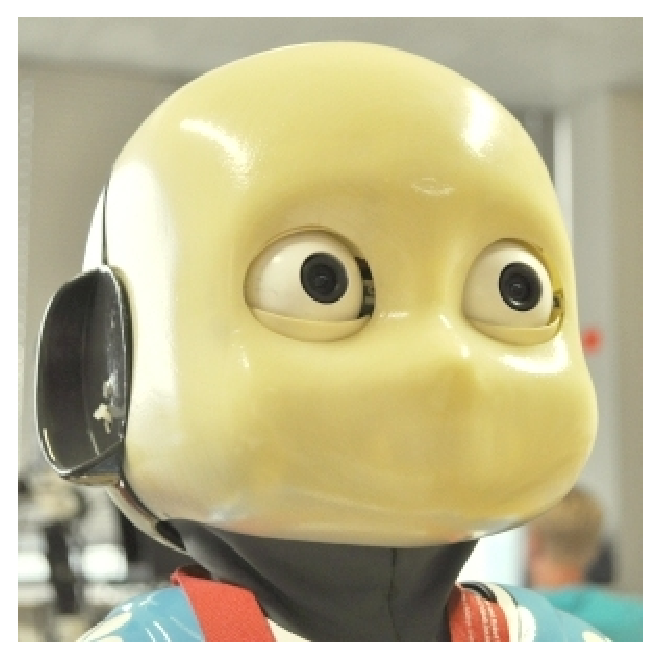
\includegraphics[width=0.4\columnwidth]{images/intro/chica_head} & 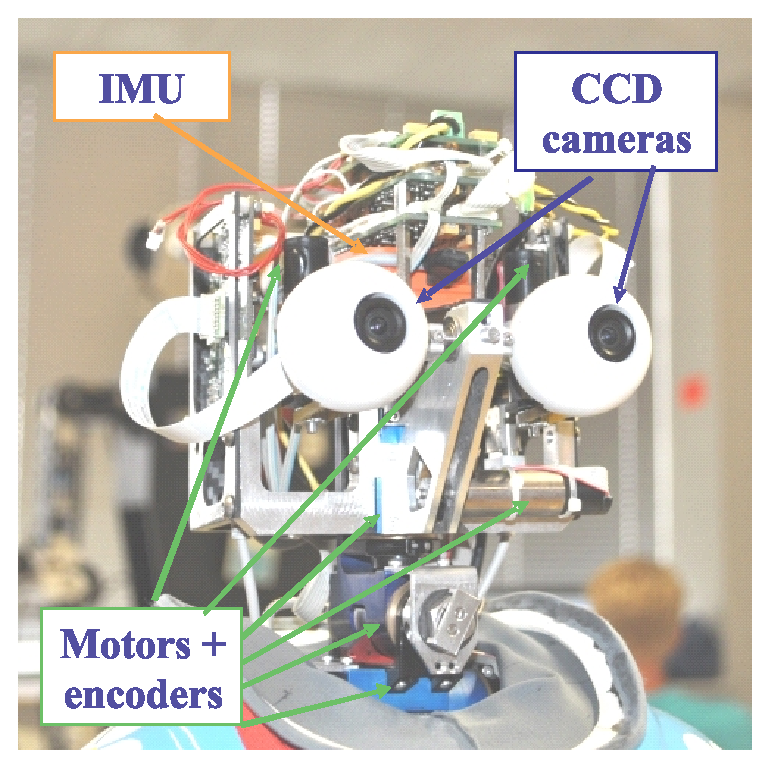
\includegraphics[width=0.4\columnwidth]{images/intro/chica_head_devices}\\
  a) iCub head & b) Actuators and sensors \\
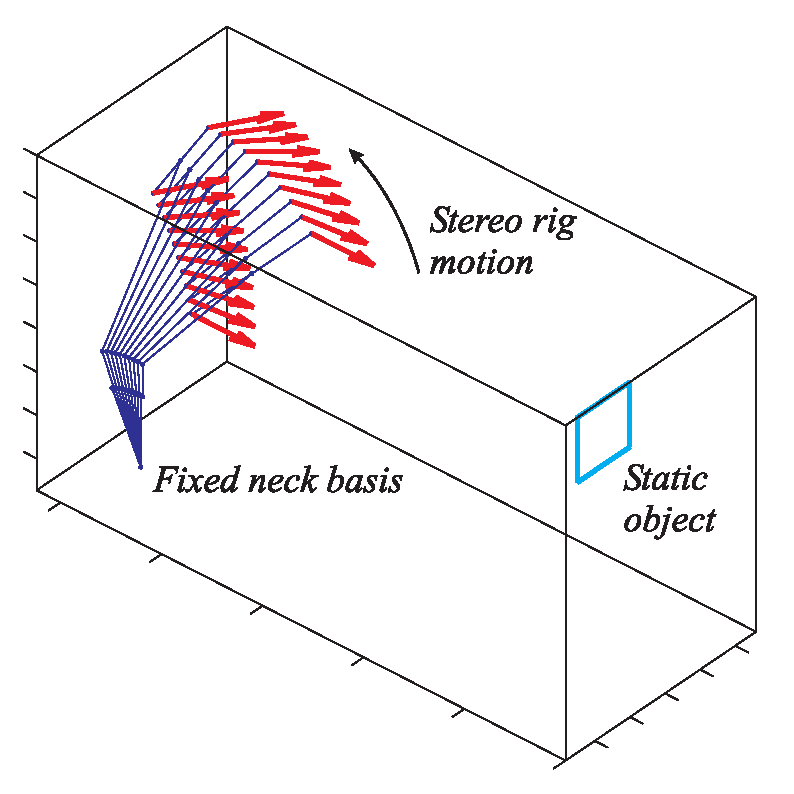
\includegraphics[width=0.4\columnwidth]{images/intro/cam_sim_err_localiz_v2} & 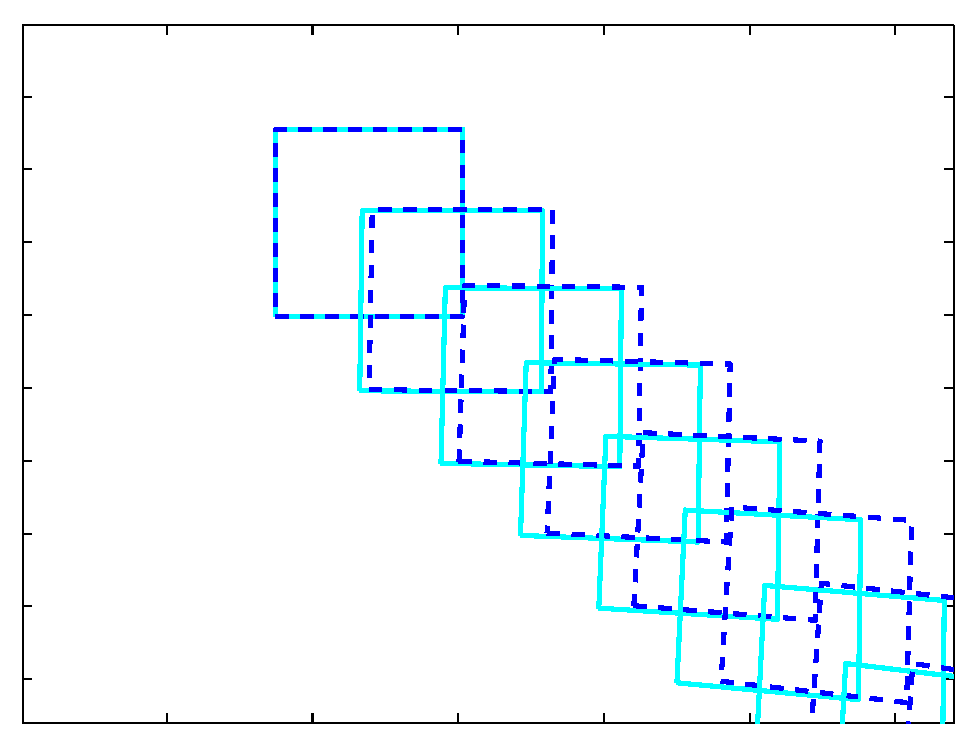
\includegraphics[width=0.4\columnwidth]{images/intro/cam_sim_err_5deg}\\
  c) Sample cameras motion & d) $5\deg$ offsets
\end{tabular}
\caption{The iCub head used in this work (a). Sensors and actuators in the iCub head encompass two cameras, six motors with relative encoders, and one IMU (b). Example of a trajectory of the stereo cameras (red arrows), that observe an object in the scene (cyan square), to demonstrate the effect of the offsets in the expected perception (c). Images of the cyan square seen by the left camera and expected perception (dashed lines) when all the joints have $5\deg$ offsets (d).}
\label{fig:intro_figure}
\end{figure}

Using absolute encoders in the joints may seem as solution for this specific problem. However it is not guaranteed the zero position of each joint matches the absolute zero of the kinematic model, mostly because many of these platforms are hand mounted. Misalignment due to mounting errors of the sensors need to be detected and corrected before the platform is used otherwise there will be undesirable offsets in the position of the end-effector when performing the tasks it was designed for, as seen in figure \ref{fig:intro_figure}c). In this example, stereo cameras are observing a scene while performing a trajectory with $5\deg$ offsets in all their joints. We can clearly see in figure \ref{fig:intro_figure}d) the misalignment between the real position of the scene object (solid square) and its prediction given by the uncalibrated kinematic model. Having misaligned absolute encoders in the motor joints is similar to have relative ones, except that for the first case the offsets are always constant requiring only a single calibration (while relative encoders have to be calibrated every time the motors are switched on).

%Assuming the robot has absolute encoders that were perfectly mounted in the motor joints, the continuous use of the robotic platform generates drift in some of the joints, mainly on those supporting most of the platform's weight which can not be detected solely using information from the encoders. Common robotic heads present relative encoders, misaligned absolute encoders and slow drifts in mechanical positions due to wear and impacts. 

With this work we aim at combining information from the different embedded sensors and non-linear filtering techniques to completely calibrate a humanoid robot head in a real-time fashion. The proposed method calibrates entirely the kinematic structure of the system despite these problems, at a software level.

The outline of the paper is the following. In Section \ref{sec:head_calibration_system} we introduce the robotic head model that was adopted and illustrate the problem of having offsets in the motor joints; in Section \ref{sec:calibration_methodology} we present the calibration methodology that aims to estimate the offsets in the motor joints by using non-linear filtering techniques; Section \ref{sec:experiments_results} contains the experiments we have performed to validate and test the proposed solution, either in simulation and with a real robotic head, namely the iCub.


\subsection{Related Work}

% -- This section needs work. A journal, as compared to a conference, requires comprehensive well developed related work.

% Start by the "body schema". Cite a seminal work, in order to show it is a well known, classical, problem / objective, which will be widespread due to mass consumer market

% current line of refs: Hersch08, Cantin10, Tworek08, Santos10

Seminal works addressed the robot self-calibration problem as non-linear parameter estimation problems given sufficient input data from the robot sensory system. For instance, the so-called Body Schema, a denomination for the set of kinematic parameters that form the robot model, including link lengths and angles in addition to joints offsets, have been estimated with local optimization methods given appropriate initializations. 

In \cite{Hersch08} the authors present an online learning system for the body schema of the Hoap3 robot, a humanoid robotic platform with 24 degrees of freedom (DOF). The system uses information from the propriosensors and from stereo vision to correct and calibrate its internal model, by tracking its end-effectors using color markers. Although the authors show good results in simulation, for the considered approach, they recognize it is difficult to implement such a solution in a real robot with many DOF since it would take a large amount of time for the robot to explore all its joints space, by randomly moving its end-effectors. In particular, for some of its end-effectors the acquired information may be insufficient due to lack of direct visibility (the robot may not be able to always observe its feet). The random exploration of the whole joints space is widely time-consuming and may not provide enough information for the system to correctly converge. An intelligent exploration of this space could highly improve the calibration results while reducing the total calibration time. 

The authors in \cite{Cantin10} present an online active learning algorithm for the body schema of a robot that uses markers in its end-effectors. However, the main contribution of that work resides in the way the robot explores its joints space. This exploration, contrary to other approaches using active learning techniques, is not random but selective in the acquired observation. The robot will only get observations that could actually improve its calibration and explore areas where uncertainty remains high. The accuracy and speed improvement by using this technique is considerable when comparing with a passive approach where the robot randomly explored its joints space. It is of utmost importance to understand if an observation will actually add useful information to the system or simply act as noise. 

In the work described in \cite{Tworek08} the authors present a kinematic calibration system for a pan-tilt structure with a camera as its end-effector. The system estimates the homographies between consecutive time-instants by tracking points on the images. This method allows the calibration of the joint angles offsets that were present at startup due to relative encoders. Robotic platforms with relative encoders require a kinematic calibration before any operation and in these cases, calibration time is crucial. The authors in \cite{Santos10} present a kinematic calibration algorithm for a robotic head, similar to the one used in our thesis. This robotic head is equipped with relative encoders and they propose a solution to estimate the offsets of each joint, from the neck base to each of the eyes. The problem is separated into two sub-problems that are solved using different methods, more suitable for each case. To calibrate the head the authors use information from the inertial sensor in order to find the joints offsets that enables the alignment of the head with the robot's body. To calibrate the eyes the authors used the same approach as in \cite{Tworek08}. None of the implemented methods take noise into consideration which may lead to erroneous estimations. Moreover, these approaches were not designed to be used in an online manner and can not respond or adapt to changes that may occur during operation. Due to heavy use these platforms usually have slow mechanical drifts in their motor shafts due to wear, impact and strain that deform the parts, where the encoders can not provide any measurements. An online calibration system can detect these changes and adapt its estimates along time as we will show in this thesis.

From the literature we can see that most solutions require special markers to calibrate the robotic platforms or simply cannot calibrate it in an online fashion. In this work we present a full calibration system for a robotic head platform that aims to calibrate its kinematic model in an online fashion, without any special markers, using only natural information from the environment and measurements from its embedded sensors. Our system can be left running during the whole operation of the robot, in order to adapt to any changes that may occur.


%\section{Head Calibration System}
\section{Robot Head Model}
\label{sec:head_calibration_system}

The robot head is represented by a kinematic chain formed by multiple rotation joints serially coupled (see figure \ref{fig:head_kinematic_model_prob_form}a). 

\begin{figure}
\centering
    \centering
    \begin{tabular}{ccc}
    \includegraphics[width=0.3\columnwidth]{images/Head_Kinematic_Model_v2} & &
    \includegraphics[width=0.15\columnwidth]{images/offset_model} \\
    a) & & b)
    \end{tabular}
    \caption{The head kinematic model; a) the corresponding serial chain of joints, from the neck base $\left\{ 0\right\} $ to the eyes final joints $\left\{ 4\right\} $ and $\left\{ 5\right\} $; b) a cross section of a joint $\left\{ i\right\} $ showing the relation between the encoder measurement $e_i$ and the offset $\delta_i$ in the calibrated joint angle $\theta_i$}
\label{fig:head_kinematic_model_prob_form}
\end{figure}

Each joint $i$ can rotate by an angle $\theta_i$ around its axis of rotation. In a calibrated internal model, $\theta_{i}$ corresponds to the exact measurement given by the encoder sensor, $e_i$. However if the internal model is not properly calibrated, there is an offset $\delta_{i}$ that must be considered and the angle $\theta_{i}$ becomes a linear combination of the encoder measurement and the offset, as seen in figure \ref{fig:head_kinematic_model_prob_form}b), with the relation given by:

\begin{equation}
\theta_{i} = e_{i}-\delta_{i}
\label{eq:offset_relation}
\end{equation}

Let $^{i+1}R_{i}\left(\theta_{i}\right)$ represent a rotation between two consecutive joints, $i$ and $i+1$. This rotation is a function of the rotation angle $\theta_{i}$ associated to the $i$th joint. The complete rotation from a reference frame $\{n\}$ to the base of the kinematic chain $\{0\}$ is written as

\begin{equation}
^{n}R_{0}\left(\theta_{0},\ldots,\theta_{n-1}\right)={}^{n}R_{n-1}\left(\theta_{n-1}\right)\ldots{}^{2}R_{1}\left(\theta_{1}\right){}^{1}R_{0}\left(\theta_{0}\right)
\label{eq:kinematic_chain}
\end{equation}

We can easily see that an offset in one of the primary joints or the composition of multiple offsets through the kinematic chain may introduce large errors in the final orientation of its end-effector. The goal of our work is to estimate all the offsets $\delta_{i}$ so the rotation given by the kinematic model adequately reflect the real state of the system and the relation (\ref{eq:offset_relation}) holds for every considered joint.

In the case of a typical robot head equipped with an IMU and stereo cameras, which includes all the head joints from the neck base $\{0\}$ to both eyes $\{4\}$ and $\{5\}$ as seen in figure \ref{fig:head_kinematic_model_prob_form}a), we want to find the offsets defining the head's absolute zero position, with both cameras pointing to the front (projection planes orthogonal to the floor) and a gravity vector reading, given by the IMU, corresponding to a vertical vector pointing down.

\subsection{Observability Analysis}

The model presented in (\ref{eq:kinematic_chain}) is able to describe any kinematic chain from a combination of multiple rotation matrices, one per each joint. However, this model presents observability problems when consecutive joints are rotating about the same rotation axis, since their rotation becomes coupled. Let's consider the following example where a kinematic chain has two consecutive joints rotating about the $x$ axis, by angles of $\alpha$ and $\beta$. 

\begin{equation}
R\left(\alpha,\beta\right)=R_{x}\left(\alpha\right)R_{x}\left(\beta\right)
\label{eq:rotation_observability}
\end{equation}
with $R_{x}\left(\alpha\right)$ given by:

\begin{equation}
R_{x}\left(\alpha\right)=\left[\begin{array}{ccc}
1 & 0 & 0\\
0 & \cos\left(\alpha\right) & -\sin\left(\alpha\right)\\
0 & \sin\left(\alpha\right) & \cos\left(\alpha\right)
\end{array}\right]
\end{equation}
(analogous for $R_{x}\left(\beta\right)$).

After the product, equation (\ref{eq:rotation_observability}) becomes:

\begin{equation}
R\left(\alpha,\beta\right)=\left[\begin{array}{ccc}
1 & 0 & 0\\
0 & \cos\left(\alpha+\beta\right) & -\sin\left(\alpha+\beta\right)\\
0 & \sin\left(\alpha+\beta\right) & \cos\left(\alpha+\beta\right)
\end{array}\right]
\end{equation}
where we applied trigonometric relations to simplify the notation. In the final rotation $R\left(\alpha,\beta\right)$, $\alpha$ and $\beta$ are coupled. Considering $\theta=\alpha+\beta$, this coupling behaviour means any value of $\theta$ can be obtained from an infinite number of linear combinations of $\alpha$ and $\beta$. Having infinite possibilities for both angles, the system can't estimate the real offsets for each joint. However, the differential between the two is always constant and by fixing one of the joints (assuming it has no offset), it is still possible estimate the offset for the other joint.

\section{Calibration Methodology}\label{sec:calibration_methodology}

The base of our calibration system is an Implicit Extended Kalman Filter (IEKF) since part of our observations' predictions can not be directly obtained from the system state only. In the following sections we will explain the IEKF in more detail and introduce the dynamic and observation models for our filter considering the nature of the problem.

\subsection{Implicit Extended Kalman Filter}

The Implicit Extended Kalman Filter (IEKF) is a variation of the Extended Kalman Filter (EKF) \cite{Ribeiro04} where the measurements take the form of an implicit constraint that is a function of both the system state and the sensors observations. Soatto introduced this variation in \cite{Soatto96,Soatto96b} as a way to estimate the motion of a moving camera using the epipolar constraint \cite{Hartley04} as the system's measurements.

\subsubsection{State and Observation Model}

In a generic IEKF the system assumes its state evolves according to a certain dynamic model (identical to the EKF's), linear or not, considering it has no inputs, as:

\begin{equation}
x^{k+1}=f^{k}\left(x^{k}\right)+w^k
\label{eq:iekf_generic_prediction}
\end{equation}
where $f^k$ corresponds to the state transition function, $x^{k}$ and $x^{k+1}$ denote the system states at time instants $k$ and $k+1$ and $w^{k}\sim \mathcal{N}\left(0,Q^{k}\right)$ is an additive zero mean Gaussian noise with covariance $Q^{k}$.

In the standard EKF the measurements are explicit functions of the system state $x$ and they can be obtained from a measurement model of the form:

\begin{equation}
y^{k+1} = h^{k+1}\left(x^{k+1}\right) + v^{k+1}
\label{eq:iekf_generic_measurement_y}
\end{equation}
where $h^{k+1}$ corresponds to the measurement function, with $v^{k+1}\sim \mathcal{N}\left(0,R^{k+1}\right)$ as an additive zero mean Gaussian noise with covariance $R^{k+1}$. However in the IEKF, the filter measurement equation takes the form of a constraint $z$ that must be fulfilled and is an implicit function of both the system state $x$ and the physical measurements from the sensors, $y$:

\begin{equation}
z^{k+1} = h^{k+1}\left(x^{k+1}, y^{k+1}\right) = 0
\label{eq:iekf_generic_constraint}
\end{equation}

This hybrid model is extremely useful when the system's innovation $z^{k+1}$ cannot be linearly obtained from the predicted observations and the real observations. \footnote{In the EKF $z^{k+1}$ is given by the difference between the predicted observations $\bar{y}^{k+1}=h^{k+1}\left(\bar{x}^{k+1}\right)$ and the real observations $y^{k+1}$, $z^{k+1}=\bar{y}^{k+1}-y^{k+1}$.}

\subsubsection{Prediction and Update Equations}

The IEKF, like the EKF, is a two-step procedure with a prediction and an update step. In the prediction step, the system state is propagated using the dynamic model described in (\ref{eq:iekf_generic_prediction}):

\begin{equation}
\bar{x}^{k+1}=f^{k}\left(\hat{x}^{k}\right)
\label{eq:iekf_generic_state_prediction}
\end{equation}
where $\hat{x}^{k}$ corresponds to the estimate of $x$ from the previous time instant, with the previous state covariance matrix estimation $\hat{P}^{k+1}$ being propagated and predicted using the standard filter equation:

\begin{equation}
\bar{P}^{k+1}=\mathcal{F}^{k}\hat{P}^{k}\left(\mathcal{F}^{k}\right)^{T}+Q^{k}
\label{eq:iekf_generic_state_cov_prediction}
\end{equation}
where $\mathcal{F}^{k}$ is the Jacobian of $f^{k}$ obtained by linearizing the function, evaluated at the previous state estimate $\hat{x}^{k}$:

\begin{equation}
\mathcal{F}^{k}=\left.\frac{\partial f^{k}}{\partial x}\right|_{x=\hat{x}^{k}}
\end{equation}

In the update step, the predicted filter measurement $\bar{z}^{k+1}$ is used as the filter's innovation and is obtained from the current state prediction $\bar{x}^{k+1}$ and the observations $y^{k+1}$ :

\begin{equation}
\bar{z}^{k+1} = h^{k+1}\left(\bar{x}^{k+1}, y^{k+1}\right)
\label{eq:iekf_generic_measurement}
\end{equation}

The final state update $\hat{x}^{k+1}$, given the previous measurement prediction, takes the form:

\begin{equation}
\begin{array}{ccc}
\hat{x}^{k+1} & = & \bar{x}^{k+1}+K^{k+1}\left(z^{k+1}-\bar{z}^{k+1}\right)\\
 & = & \bar{x}^{k+1}-K^{k+1}\bar{z}^{k+1}\end{array}
\end{equation}
where the matrix $K^{k+1}$ corresponds to the Kalman gain (note that as described in (\ref{eq:iekf_generic_constraint}), $z^{k+1}=0$). The update of the state covariance matrix $\hat{P}^{k+1}$ is given by:

\begin{equation}
\begin{array}{ccc}
\hat{P}^{k+1} & = & \left(I-K^{k+1}H^{k+1}\right)\bar{P}^{k+1}\left(I-K^{k+1}H^{k+1}\right)^{T}\\
 &  & +K^{k+1}\tilde{R}^{k+1}\left(K^{k+1}\right)^{T}\end{array}
\end{equation}
where the Kalman gain matrix $K^{k+1}$ is obtained as:

\begin{equation}
K^{k+1}=\bar{P}^{k+1}(H^{k+1})^T\left(H^{k+1}\bar{P}^{k+1}\left(H^{k+1}\right)^{T}+\tilde{R}^{k+1}\right)^{-1}
\label{eq:kalman_gain}
\end{equation}

In the previous equations, $H^{k+1}$ corresponds to the Jacobian of $h^{k+1}$ obtained through linearization of the function, evaluated at the current state estimate $\hat{x}^{k+1}$:

\begin{equation}
H^{k+1}=\left.\frac{\partial h^{k+1}}{\partial x}\right|_{x=\hat{x}^{k+1}}
\end{equation}
and $\tilde{R}^{k+1}$ is the first-order approximation of the covariance of the noise in the implicit measurement constraint. The noise in the sensors measurements $R^{k+1}$ must be propagated to the measurement function $h^{k+1}$, in order to map the noise in the implicit measurements \cite{Soatto96}. The relation between this covariance noise and the covariance noise of the sensors measurements $R^{k+1}$ is given by:

\begin{equation}
\tilde{R}^{k+1}=D^{k+1}R^{k+1}\left(D^{k+1}\right)^{T}
\label{eq:implicit_measurements_cov}
\end{equation}
where $D^{k+1}$ is given by:

\begin{equation}
D^{k+1}=\left.\frac{\partial h^{k+1}}{\partial y}\right|_{y=y^{k+1}}
\end{equation}

\subsection{Proposed Architecture}

Our system assumes the robotic platform under calibration is equipped with three types of sensors: an inertial measurement unit (IMU) that generates linear acceleration and angular velocities measurements, motor encoders that provide the motor angles of the joints and stereo cameras that generate real images of the world. %If, by any chance, one of these sensors stops working, the system is still able to calibrate the robotic head using the other sensors up to the kinematic location of the failed sensors. 

In the following implementation we will assume the base of the kinematic chain is static and aligned with gravity in a planar horizontal surface, the world is static and infinite (all the objects seen by the cameras are at a very large distance) and there are no mounting errors of the IMU nor the cameras which is a good approximation for the level of calibration we aim for the head.

\subsubsection{State Transition Model}

The system state $x$ is given by:

\begin{equation}
x=\left[\begin{array}{ccc}
\delta_{0} & \ldots & \delta_{N-1}\end{array}\right]\in\mathbb{R}^{N}
\end{equation}
where $\delta_{i}$ corresponds to the $i$th joint offset, represented in figure \ref{fig:head_kinematic_model_prob_form}a). These offsets are assumed to be constant over time, thus the state transition equation $f$ simply propagates the previous values. To allow for small changes of the values over time, e.g. due to mechanical wear or slippage, we allow for some state transition noise $w^k$.

The system state transition model $f$ is therefore:
%
\begin{equation}
\begin{array}{c}
x^{k+1}=f\left(x^{k}\right)+w^{k}
\end{array}
\label{eq:F}
\end{equation}
%
where $f\left(x^{k}\right)=x^{k}$ and $w^k\sim \mathcal{N}\left(0,Q^k\right)$ is the state transition noise assumed to be a zero mean Gaussian with covariance matrix $Q^k$. The system can be adapted to be more or less sensitive to variations in the estimate of the offsets by changing this covariance matrix.

\subsubsection{Observation Model}

The considered robotic platforms are equipped with three types of sensors: an IMU, cameras and encoders. From these we can obtain four types of different measurements, depending on the sensor we are considering.

The IMU provides measurements for linear accelerations
\begin{equation}
y_{A}^{k+1}=\left[a_{x}^{k+1},a_{y}^{k+1},a_{z}^{k+1}\right]^{T}\in{\mathbb{R}}^{3}
\end{equation}
and angular velocities
\begin{equation}
y_{W}^{k+1}=\left[w_{x}^{k+1},w_{y}^{k+1},w_{z}^{k+1}\right]^{T}\in{\mathbb{R}}^{3}
\end{equation}
for the three principal axes on which it is mounted. We assume that the linear accelerations measured by the IMU correspond to the effects of the gravity vector decomposed in the three components of $x$, $y$ and $z$ affected by sensor noise, which is valid for slow movements of the robotic head. 

The cameras provide $M$ image features represented by their image coordinates

\begin{equation}
p_{i}=\left[u_{i},v_{i}\right]\in{\mathbb{R}}^{2}
\end{equation}
in pixel units. Here we are interested in image movement induced by the joints, hence we always consider a pair of consecutive frames as measurements

\begin{equation}
y_{F}^{k}=\left[p_{0}^{k},\ldots,p_{M-1}^{k}\right]^{T}\in{\mathbb{R}}^{2M}
\end{equation}
and
\begin{equation}
y_{F}^{k+1}=\left[p_{0}^{k+1},\ldots,p_{M-1}^{k+1}\right]^{T}\in{\mathbb{R}}^{2M}.
\end{equation}

The encoders provide $N$ measurements of the relative position of the joints in two consecutive time instants $k$ and $k+1$, 
\begin{equation}
y_{E}^{k}=\left[e_{0}^{k},\ldots,e_{N}^{k}\right]^{T}\in{\mathbb{R}}^{N}
\end{equation}
and 
\begin{equation}
y_{E}^{k+1}=\left[e_{0}^{k+1},\ldots,e_{N}^{k+1}\right]^{T}\in{\mathbb{R}}^{N}
\end{equation}
where $e_i$ corresponds to the $i$th relative encoder measurement as represented in figure \ref{fig:head_kinematic_model_prob_form}b). The encoders usually work at a very high frequency ($1000$Hz), much higher than the IMU ($100$Hz) or the cameras ($30$Hz), in our case corresponding to the slowest sensor. For this reason, the IMU and cameras are responsible for setting the sampling instants where the measurements are acquired since there are always available encoders measurements. Considering the IMU works at a higher frequency than the cameras, its measurements are acquired in between two camera measurements.

In order to predict all the sensors measurements the absolute value of each joint is needed to compute the complete rotation $^iR_0$ from the base of the kinematic chain to the reference frame $i$ where each sensor is mounted. Collecting equations (\ref{eq:offset_relation}) in vector form, the absolute values of the joints $\Theta$ for both time instants $k$ and $k+1$ are given by
\begin{equation}
\begin{array}{c}
\Theta^{k}=y_{E}^{k}-\bar{x}^{k+1}\\
\Theta^{k+1}=y_{E}^{k+1}-\bar{x}^{k+1}
\end{array}
\label{Eq:Encoders_real}
\end{equation}
where the current offsets prediction $\bar{x}^{k+1}$ was used in the two cases since the offsets, ideally, should be constant over time.

Considering the IMU is mounted on reference frame $I$ we represent the base to IMU coordinate roto-translation by $^{I}R_{0}\left(\Theta^{k+1}\right)$. The prediction of the linear accelerations measurements $\bar{y}_{A}^{k+1}$ are obtained by mapping the world constant gravity vector by this rotation: 

\begin{equation}
\bar{y}_{A}^{k+1}={}^{I}R_{0}\left(\Theta^{k+1}\right).\left[0,-G,0\right]^{T}
\label{eq: za_pred}
\end{equation}
where $G$ corresponds to the standard gravity value $9.806m.s^{-2}$. Note the negative sign since the accelerometer measures the gravity reaction.

The predictions of the angular velocities measurements $\bar{y}_{W}^{k+1}$ are computed from the derivative of the IMU reference frame, here approximated by the change of this reference frame between two consecutive time instants divided by the change in time. Since the base of the robotic platform does not move these velocities are given by
\begin{equation}
\bar{y}_{W}^{k+1}=Rodrigues^{-1}\left(^{I}R_{0}\left(\Theta^{k+1}\right).\left(^{I}R_{0}\left(\Theta^{k}\right)\right)^{-1}\right)/dT
\label{eq: zw_pred}
\end{equation}
where the inverse Rodrigues function \footnote{The inverse Rodrigues formula provides a closed form solution to the Lie logarithm function on the rotation Lie group.} \cite{Rodrigues40} provides the instant angular change and $dT$ is the time interval between the two encoder measurements.

To obtain the image features predictions $\bar{y}_{F}^{k+1}$ for a camera in reference frame $C$ we need as well two consecutive orientations of this reference frame. We are approximating the world as having all the points at infinity, given the low parallax between two consecutive images. Considering this approximation, we assume that all the image features will only be affected by a pure rotation. The prediction of the image features is obtained as:
\begin{equation}
\bar{y}_{F}^{k+1}=\left[\bar{p}_{0}^{k+1},\ldots,\bar{p}_{M-1}^{k+1}\right]^{T}
\end{equation}
where the $i$th image feature prediction $\bar{p}_{i}^{k+1}$ is given by
\begin{dmath}
\lambda\left[\bar{p}_{i}^{k+1},1\right]^{T}={}^{C}R_{0}\left(\Theta^{k+1}\right).\left(^{C}R_{0}\left(\Theta^{k}\right)\right)^{-1}.\left[p_{i}^{k},1\right]^{T}
\label{eq: zf_pred}
\end{dmath}
where $\lambda$ is a scale factor. This equation provides a set of constraints, two for each image feature, that needs to be satisfied by the measurements $y_F^{k+1}$ in the Implicit Kalman Filter Formulation.

Since the IMU seldomly works at the same frequency as the image acquisition sensors, these readings are usually not simultaneously available. Hence at each time step we either have an IMU observation or an image observation which needs to be filtered. For the case where we only have IMU observations, the system measurements constraint $\bar{z}^{k+1}$, obtained from the measurements function $h^{k+1}$ as described in equation (\ref{eq:iekf_generic_measurement}) is, at each time step $k$:

\begin{dmath}
\bar{z}^{k+1}=h^{k+1}\left(\bar{x}^{k+1},y_{A}^{k+1},y_{W}^{k+1},y_{E}^{k},y_{E}^{k+1}\right)=\left[\begin{array}{c}
\bar{z}_{A}^{k+1}\\
\bar{z}_{W}^{k+1}
\end{array}\right]+\tilde{v}_{I}^{k+1}
\end{dmath}
with
\begin{dmath}
\begin{array}{c}
\bar{z_{A}}^{k+1}=y_{A}^{k+1}-\bar{y}_{A}^{k+1}\left(y_{E}^{k},y_{E}^{k+1}\right)\\
\bar{z_{W}}^{k+1}=y_{W}^{k+1}-\bar{y}_{W}^{k+1}\left(y_{E}^{k},y_{E}^{k+1}\right)
\end{array}
\label{eq:z_imu}
\end{dmath}
where $\tilde{v}_I^{k+1}\sim \mathcal{N}\left(0,\tilde{R}_I^{k+1}\right)$ is the observation noise of the implicit measurement constraint in case of IMU, assumed to be a zero mean Gaussian with covariance matrix $\tilde{R}_I^{k+1}$, obtained using equation (\ref{eq:implicit_measurements_cov}) applied to the covariance matrix $R_I^{k+1}$, representing the noise of the IMU and encoders' observations. For the case where we only have image observations, the system measurements constraint $\bar{z}^{k+1}$, is given by:

\begin{dmath}
\bar{z}^{k+1}=h^{k+1}\left(\bar{x}^{k+1},y_{F}^{k},y_{F}^{k+1},y_{E}^{k},y_{E}^{k+1}\right)=\begin{bmatrix}\bar{z}_{F}^{k+1}\end{bmatrix}+\tilde{v}_{C}^{k+1}
\end{dmath}
with
\begin{dmath}
\bar{z_{F}}^{k+1}=y_{F}^{k+1}-\bar{y}_{F}^{k+1}\left(y_{E}^{k},y_{E}^{k+1}\right)
\label{eq:z_image}
\end{dmath}
where $\tilde{v}_C^{k+1}\sim \mathcal{N}\left(0,\tilde{R}_C^{k+1}\right)$ is the observation noise of the implicit measurement constraint in case of image measurements, assumed to be a zero mean Gaussian with covariance matrix $\tilde{R}_C^{k+1}$, obtained using equation (\ref{eq:implicit_measurements_cov}) applied to the covariance matrix $R_C^{k+1}$, representing the noise of the cameras and encoders' observations.. Note the dependency of $\bar{y}_{A}^{k+1}$, $\bar{y}_{W}^{k+1}$ and $\bar{y}_{F}^{k+1}$ on $y_{E}^{k}$ and $y_{E}^{k+1}$, reason why we used an IEKF, even though in this case the constraint from equations (\ref{eq:z_imu}) and (\ref{eq:z_image}) appears to be "linear" in its corresponding variables. In fact, it is highly non-linear considering the observations predictions process, already explained, which depends both on the system's state (offsets) and the real observations from the encoders.

The constraint $\bar{z}^{k+1}$ represents the Implicit Kalman filter's innovation functionand by using this function as the filter's innovation, the system is able to estimate all the offsets that set the absolute zero position for each joint, thus calibrating the entire kinematic model.
%\section{Experiments and Results}\label{sec:experiments_results}

In this section we will evaluate the proposed architecture for the head calibration system. We will perform simulated and real experiments to evaluate the system in terms of its accuracy and repeatability. The real experiments were performed using the iCub robotic platform, \cite{Metta08}, more specifically the head \cite{Beira06}. The iCub was developed in the context of the EU project RobotCub and was adopted by more than 20 laboratories worldwide. The full robot has 53 DOF with the head having 6 DOF from the neck to each of the eyes, as seen in figure \ref{fig:head_kinematic_model_prob_form}a).

For each joint the robot's head is equipped with relative encoders that are extremely precise but are unable to measure the absolute zero position of the joint. The head is also equipped with an Xsens IMU that measures the linear accelerations and angular velocities at a frequency of 100Hz. This sensor is placed on top of the head right before the eyes tilt joint, $\delta_3$, as seen in figure \ref{fig:head_kinematic_model_prob_form}a). Finally the head is equipped with two Pointgrey Dragonfly cameras, that work at 30Hz and provide RGB images with VGA resolution ($640\times480$pixel). These cameras have $4.7\times3.5$mm CCD sensors and a field of view of $87.3\degree$ (horizontal) and $70.8\degree$ (vertical). The cameras are the last sensors in the kinematic chain being affected by all the joints. The intrinsic parameters of the cameras were calibrated using the Bouguet Toolbox \cite{Bouguet08} and where the radial distortion was completely eliminated. The calibrated parameters are presented in the following table:

\begin{table}
\centering
\begin{tabular}{ccc}
 \hline
 Parameter & Left Camera & Right Camera \\
 \hline
 Width (pixel) & $640$ & $640$\\
 Height (pixel) & $480$ & $480$ \\
 $f_x$ (pixel) & $332.706$ & $342.367$\\
 $f_y$ (pixel) & $382.658$ & $389.545$\\
 $c_x$ (pixel) & $348.316$ & $350.601$\\
 $c_y$ (pixel) & $241.872$ & $251.704$\\
 \hline
\end{tabular}
\caption{Intrinsic parameters of the cameras: resolution (Width and Height), focal lengths ($f_x$ and $f_y$) and optical centers ($c_x$ and $c_y$)}
\label{tab:intrinsic_parameters}
\end{table}

In order to validate the proposed architecture we performed simulated experiments where all the sensors measurements were simulated and fed to the system just like in the real case. For both cases, the simulated and real, we created several datasets. Each dataset contains information from all the sensors at every time step: the linear accelerations and angular velocities from the IMU, the motor encoders and stereo images from both cameras (or simulated image features in the simulation case).

The head calibration system was designed to calibrate the robotic head from joint $0$, corresponding to the neck tilt joint, to joint $5$, corresponding to the left eye pan joint, as seen in figure \ref{fig:head_kinematic_model_prob_form}a). Each of these encoders is unable to provide the absolute zero position of each joint, resetting the encoders values to zero every time the motors are switched off. The calibration procedure for the simulation and real case goes as follows: the motors are initialized at an arbitrary position and we start the data acquisition while randomly rotating the head, as seen in figure \ref{fig:head_calibration_procedure}. Several datasets were acquired either for the same encoders offsets and for different encoders offsets, to completely evaluate the system in terms of its accuracy and repeatability.

\begin{figure}
    \centering
    \begin{tabular}{ccc}
        \includegraphics[width=0.25\columnwidth]{images/pos_1} &  
        \includegraphics[width=0.25\columnwidth]{images/pos_2} & 
        \includegraphics[width=0.25\columnwidth]{images/pos_3} \\
        \includegraphics[width=0.25\columnwidth]{images/pos_4} &  
        \includegraphics[width=0.25\columnwidth]{images/pos_5} & 
        \includegraphics[width=0.25\columnwidth]{images/pos_6} \\
    \end{tabular}
    \caption{The head calibration procedure where the head is initialized at a random position and is rotated in order acquire data for the different experiments.}
    \label{fig:head_calibration_procedure}
\end{figure}

To initialize the system state uncertainty as well as the transition process noise we took into consideration the nature of the problem. We are estimating joint offsets that must be combined with the encoders values to provide calibrated measurements. We are initializing the system state with the first observations received from the encoders, as soon as the calibration system starts to run. For this reason, we have a large uncertainty at the beginning considering the physical limits of each joint. To ensure the system's convergence, the state's initial uncertainty must be large enough to include all the possible values the offsets could take. Therefore we initialized each offset uncertainty with a large value, $40$deg. The transition process noise was set to $0.05$deg, so it could adapt to sudden situations while keeping the estimates as constant as possible.

We analysed the noise levels that described each of the sensors' measurements, assumed to be zero mean Gaussian noise. The standard deviations values are represented in table \ref{tab:sensors_noise}.

\begin{table}
\centering
\begin{tabular}{ccc}
 \hline
 Sensor Measurement & Symbol & Std \\
 \hline
 Linear Acceleration & $\sigma_{Ra}^{0}$ & $0.0447m/s^2$\\
  Angular Velocities & $\sigma_{Rw}^{0}$ & $0.5$deg/s\\
  Encoders & $\sigma_{Re}^{0}$ & $0.028$deg\\
  Image Features & $\sigma_{Rf}^{0}$ & $2$pixel\\
 \hline
\end{tabular}
\caption{Sensors measurements noise.}
\label{tab:sensors_noise}
\end{table}

In case of the image features, for this system we used the Harris Corner Detector explained in subsection \ref{subsec:harris_corner_detector} and Normalized Cross Correlation to track features between two consecutive images. Figure \ref{fig:harris_corners_tracking} shows an example of image features acquisition and corresponding tracking.

\begin{figure}
\centering
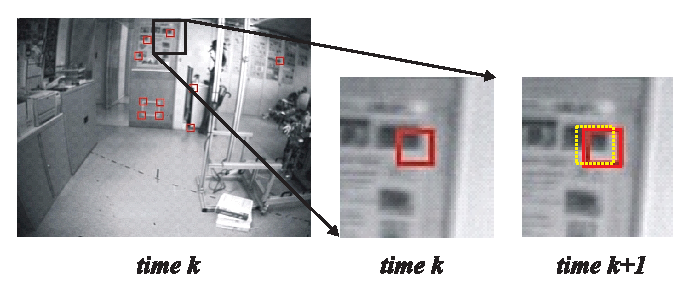
\includegraphics[width=0.75\columnwidth]{images/harris_corners_tracking}
\label{fig:harris_corners_tracking}
\caption{Example of image features acquisition and tracking using the Harris Corner Detector and Normalized Cross Correlation between two images obtained at consecutive time instants $k$ and $k+1$.}
\end{figure}

The features search in the next image was done within a limited region around the previous location of the features to reduce the computation time, assuming the images movement was small enough between two consecutive time instants.

\subsection{Simulated Experiments}\label{sec:simulated_experiments}

It is very difficult to measure the real absolute zero position of each motor joint considering there is no ground-truth for the real robot, otherwise we wouldn't require a calibration procedure. The only way to evaluate the calibration system in terms of its accuracy is by testing it with simulated experiments. Each experiment simulated the real conditions of the robot and introduced the same level of noise for each sensor according to the estimated values in table \ref{tab:sensors_noise}. It is very important to create simulated environments whose conditions are similar to the real ones.

We performed $5$ experiments where we initialized each joint with diverse offset values. For each experiment we performed $5$ trials where we simulated the rotation of the robot head. Starting from an arbitrary position, the rotation step for an $i$th joint, $\delta_i^{step}$ was sampled from a Uniform Distribution $\delta_i^{step}\sim\mathcal{U}\left(-\theta,\theta\right)$ with $\theta=0.1$deg. These values were chosen in order to best replicate the real movement that was performed by hand. Between each two steps we sampled $N=50$ virtual image features by first generating their $3D$ coordinates, within a virtual scenario ranging from $250$mm to $4000$mm, for a certain time instant and calculating their matched coordinates in the consecutive instant by using the complete roto-translation of the head. The virtual image features used as measurements were then obtained by projecting each $3D$ generated point into the corresponding virtual images. Zero-mean Gaussian noise $e$ was added to the matched image coordinates, sampled from normal distribution $e\sim\mathcal{N}\left(0,\sigma^{2}\right)$, with a standard deviation of $\sigma=2$pixel to simulate the real noise in the matching process.

The results obtained using the proposed algorithm are represented in figure \ref{fig:head_offsets_convergence} and in table \ref{tab:head_offsets_convergence}.

\begin{figure*}
\centering
\begin{tabular}{ccc}
 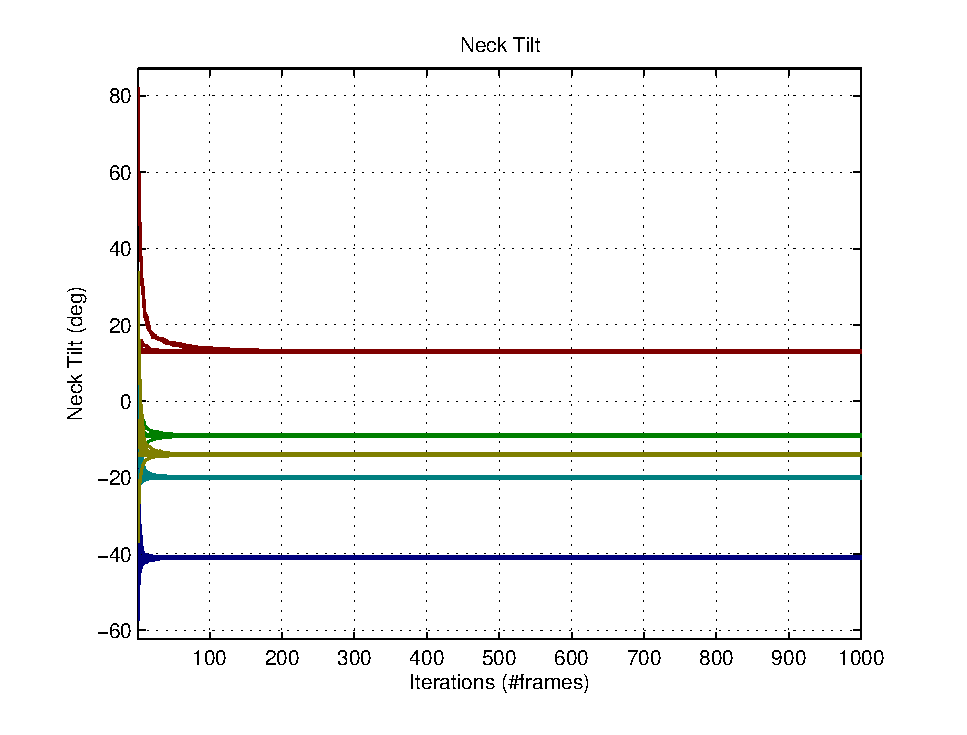
\includegraphics[width=0.32\linewidth]{images/results/neck_tilt_offsets_sim} &  
 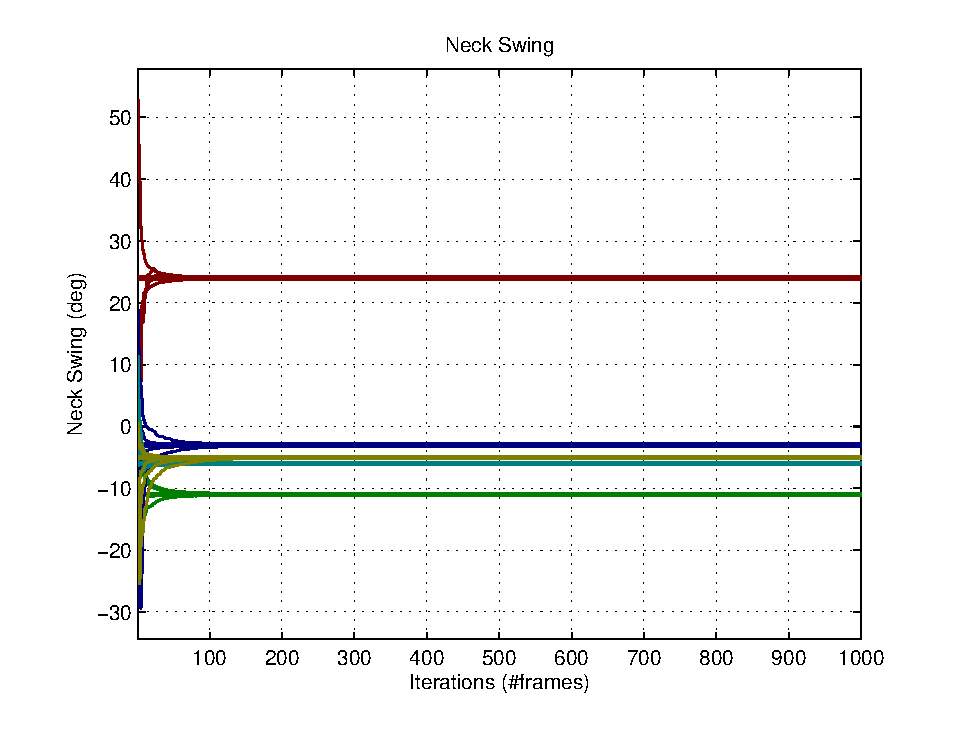
\includegraphics[width=0.32\linewidth]{images/results/neck_swing_offsets_sim} &
 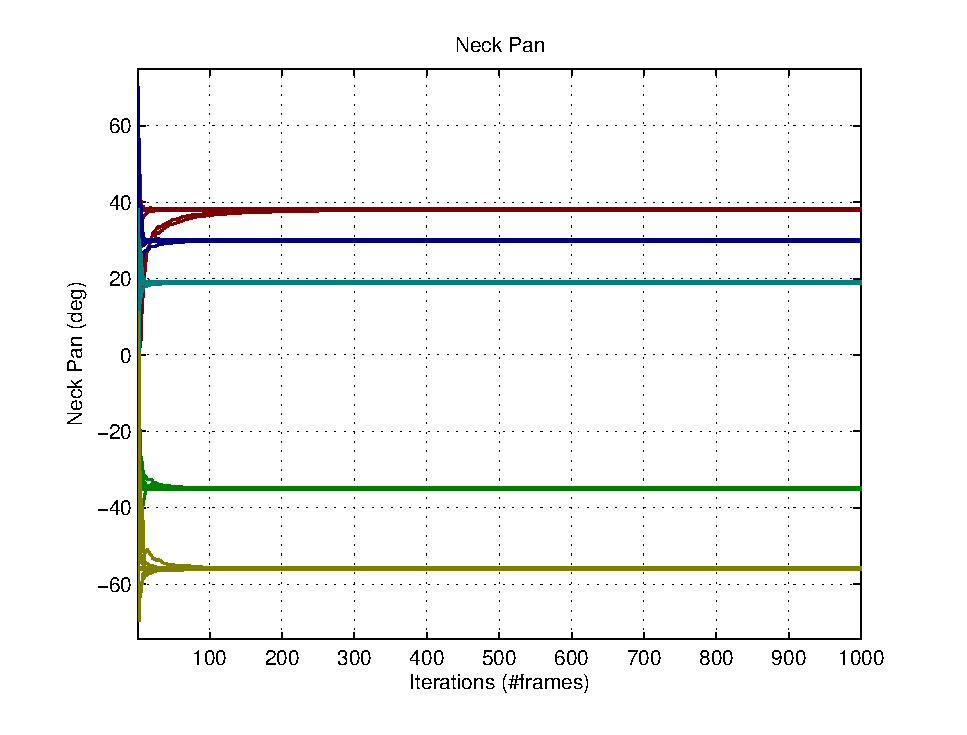
\includegraphics[width=0.32\linewidth]{images/results/neck_pan_offsets_sim} \\
  a) $\delta_0$ - Neck Tilt & b) $\delta_1$ - Neck Swing & c) $\delta_2$ - Neck Pan \\
 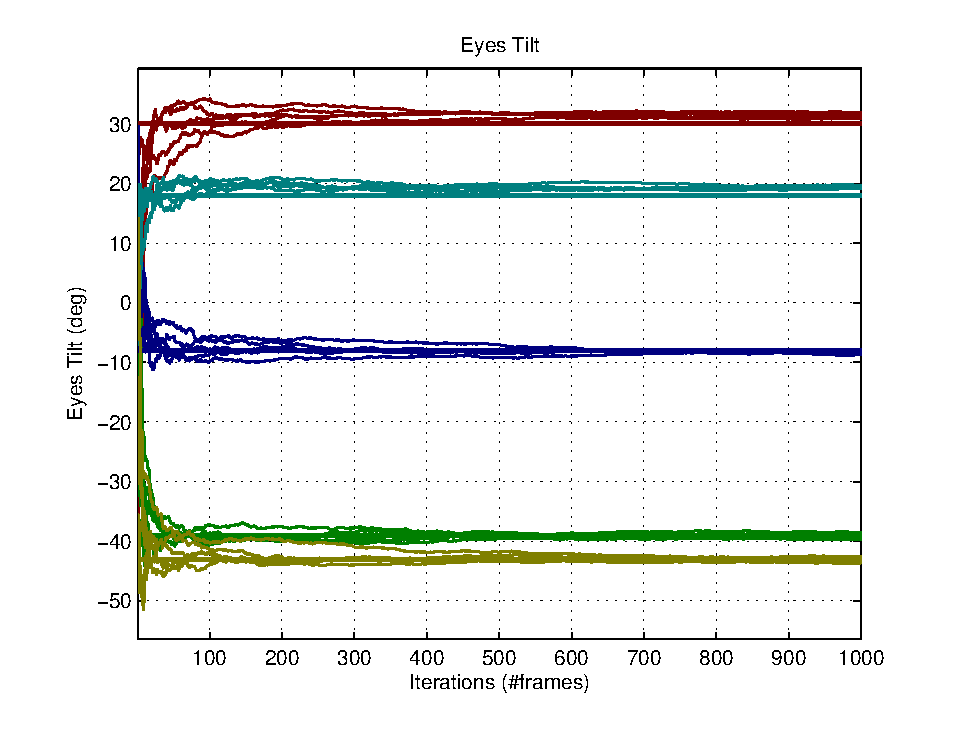
\includegraphics[width=0.32\linewidth]{images/results/eyes_tilt_offsets_sim} &
 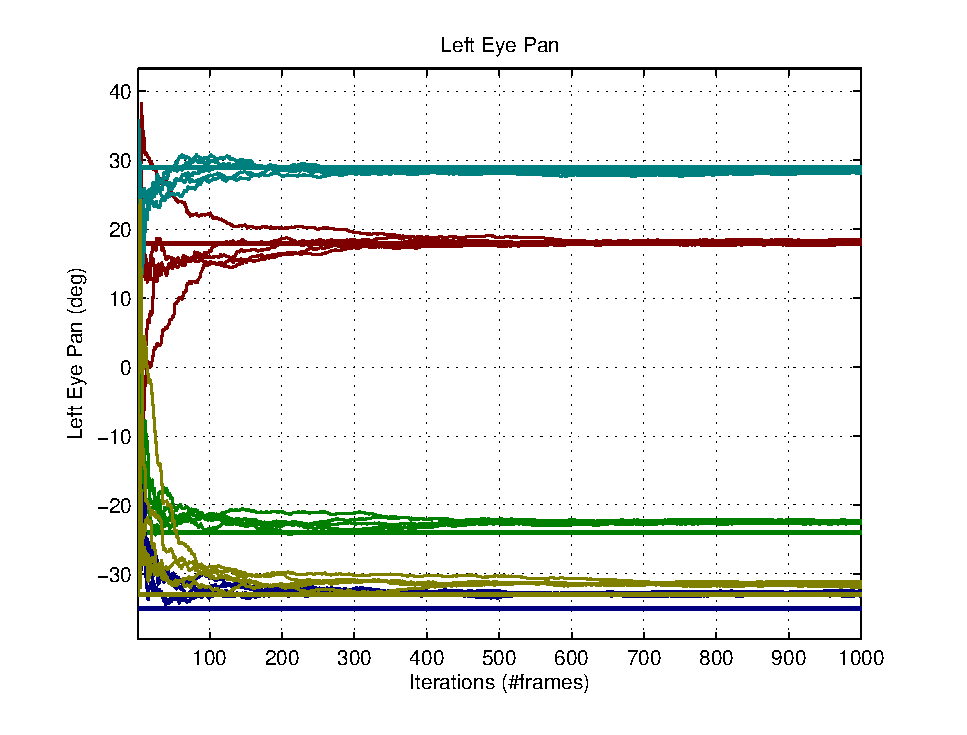
\includegraphics[width=0.32\linewidth]{images/results/left_eye_pan_offsets_sim} & 
 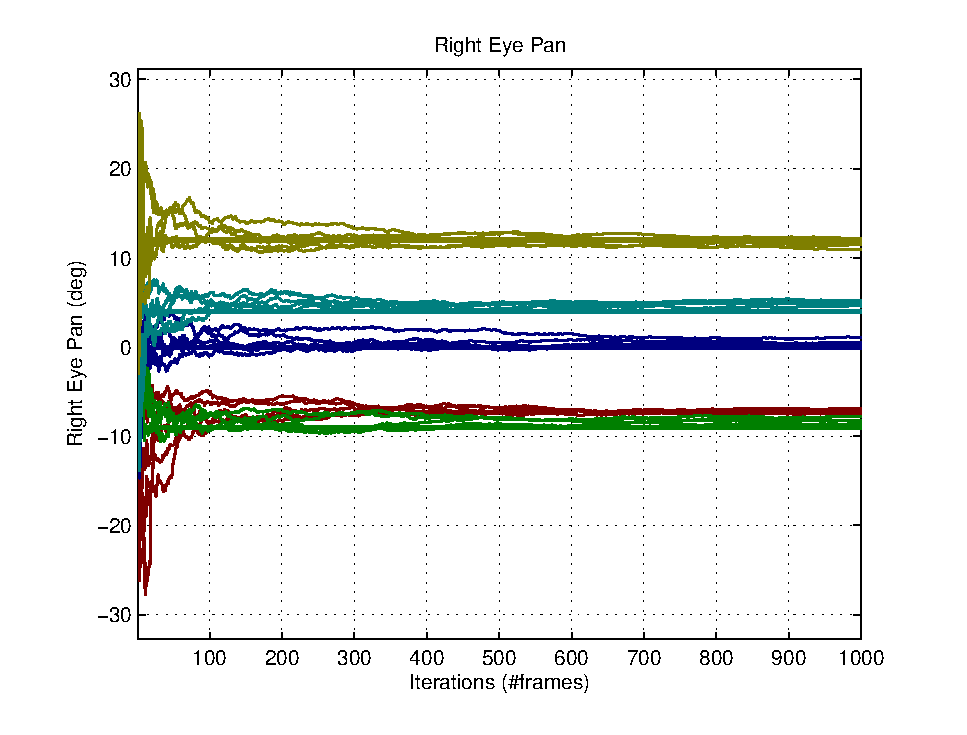
\includegraphics[width=0.32\linewidth]{images/results/right_eye_pan_offsets_sim}\\
 d) $\delta_3$ - Eyes Tilt & e) $\delta_4$ - Left Eye Pan & f) $\delta_5$ - Right Eye Pan
\end{tabular}
\caption{Head calibration offsets estimates for $5$ experiments, with $5$ trials each, in simulation: Experiment 1 (in red), Experiment 2 (in green), Experiment 3 (in blue), Experiment 4 (in cyan) and Experiment 5 (in yellow)}
\label{fig:head_offsets_convergence}
\end{figure*}

\begin{table}
\centering
\begin{tabular}{lcccccc}
 \hline
 \# Experiment & $\delta_0$(deg) & $\delta_1$(deg) & $\delta_2$(deg) & $\delta_3$(deg) & $\delta_4$(deg) & $\delta_5$(deg) \\
 \hline
$1$ (ground-truth) & 13.00 & 24.00 & 38.00 & 30.00 & 18.00 & -9.00\\
$1$ (mean) & 13.02 & 23.97 & 38.01 & 31.40 & 17.99 & -7.27\\
$1$ (std) & 0.01 & 0.01 & 0.02 & 0.29 & 0.19 & 0.16 \\
$1$ (mean error) & 0.02 & 0.02 & 0.01 & 1.40 & 0.01 & 1.72\\
 \hline
$2$ (ground-truth) & -9.00 & -11.00 & -35.00 & -39.00 & -24.00 & -9.00\\
$2$ (mean) & -9.01 & -11.02 & -34.98 & -39.11 & -22.49 & -8.36\\
$2$ (std) & 0.01 & 0.02 & 0.03 & 0.41 & 0.17 & 0.40 \\
$2$ (mean error) & 0.01 & 0.02 & 0.01 & 0.12 & 1.50 & 0.63\\
 \hline
$3$ (ground-truth) & -41.00 & -3.00 & 30.00 & -8.00 & -35.00 & 0.00\\
$3$ (mean) & -40.95 & -3.01 & 30.00 & -8.26 & -32.80 & 0.40\\
$3$ (std) & 0.01 & 0.01 & 0.02 & 0.30 & 0.25 & 0.38 \\
$3$ (mean error) & 0.04 & 0.01 & 0.01 & 0.26 & 2.19 & 0.40\\
 \hline
$4$ (ground-truth) & -20.00 & -6.00 & 19.00 & 18.00 & 29.00 & 4.00\\
$4$ (mean) & -19.97 & -6.01 & 19.00 & 19.46 & 28.34 & 4.94\\
$4$ (std) & 0.01 & 0.01 & 0.02 & 0.21 & 0.18 & 0.20 \\
$4$ (mean error) & 0.02 & 0.01 & 1.01 & 1.46 & 0.65 & 0.94\\
 \hline
$5$ (ground-truth) & -14.00 & -5.00 & -56.00 & -43.00 & -33.00 & 12.00\\
$5$ (mean) & -13.99 & -5.01 & -56.01 & -43.14 & -31.55 & 11.67\\
$5$ (std) & 0.02 & 0.01 & 0.02 & 0.38 & 0.27 & 0.46\\
$5$ (mean error) & 0.00 & 0.01 & 0.00 & 0.14 & 1.44 & 0.32\\
 \hline
\end{tabular}
\caption{The ground-truth and statistical results of the head calibration offsets estimates for $5$ experiments, with $5$ trials each.}
\label{tab:head_offsets_convergence}
\end{table}

\subsubsection{Accuracy and Repeatability}

To evaluate the system in terms of its accuracy we must compare the estimates with the ground-truth values represented in table \ref{tab:head_offsets_convergence}. As we can see the error between the real and estimated offsets is very low independently of the starting position of the head. In this case we have a maximum error of $7\%$ (or $2.19$deg) for the left eye pan joint in experiment $4$. The eyes offsets are the ones presenting the largest errors which can be explained by the approximation taken for the calibration system, where we are assuming the world is static and all points are represented at infinity which is not true and may introduce parallax errors that are compensated by the system as errors in the joint space. However we can consider this approximation is still valid for small rotations in short steps between two consecutive time instants, considering our system presents an average error of $0.99$deg for the mentioned eyes joints ($\delta_4$ and $\delta_5$). All the other joints are able to converge to its correct values with much lower errors thus proving the proposed calibration system is accurate. 

The system can converge in less than $300$ iterations, which considering the lowest sensor runs at $30$Hz and the system works in real time, corresponds to a convergence in less than $10$s. This is very important since the robot can be rapidly calibrated before operation without consuming much of the operator's time. We can see each estimate remains almost constant after convergence, even if the head is continuously rotating.

The standard deviation values represented in table \ref{tab:head_offsets_convergence} show the repeatability of the system, where it always converges to the same offsets under different operation conditions without a full reset of the encoders. This is extremely important considering the robot is being calibrated in an online fashion and it should always maintain its offsets estimates as constant as possible, in order to keep a well calibrated internal model. 

\subsection{Real Experiments}\label{sec:real_experiments}

The validation of the proposed architecture was very important before testing it in the real robot. The quality of the previous results gave us confidence to test the calibration system in the real robot. Unfortunately, in the real case, there is no ground-truth for the real offsets of the robot. Therefore we can only analyse our system in terms of its repeatability. 

We performed four experiments where we initialized the robot head at different arbitrary positions. For each experiment we performed five trials where we randomly rotated the robot head and eyes by hand during $33.33$ seconds ($1000$ iterations) so as to span most of the range of the robots joints. The estimated results are represented in figure \ref{fig:real_head_offsets_convergence} and in table \ref{tab:real_head_offsets_convergence}. We are not plotting the real encoder values during head motion since it it extremely clutter, considering each motion was unique and totally arbitrary.

\begin{figure*}
\centering
\begin{tabular}{ccc}
 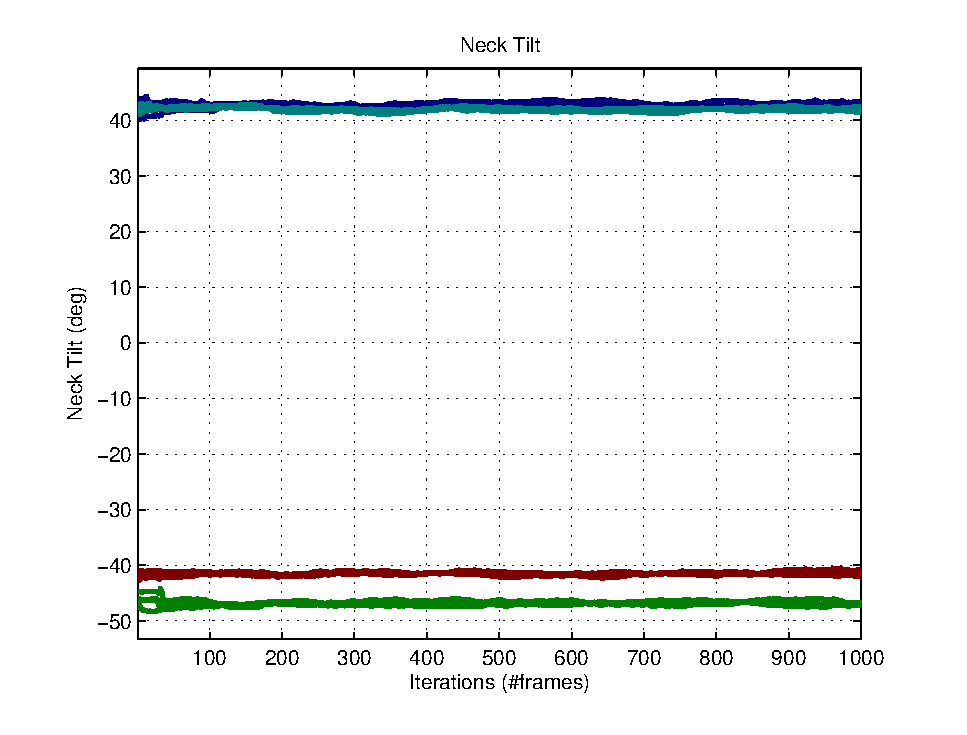
\includegraphics[width=0.32\linewidth]{images/results/neck_tilt_offsets} &  
 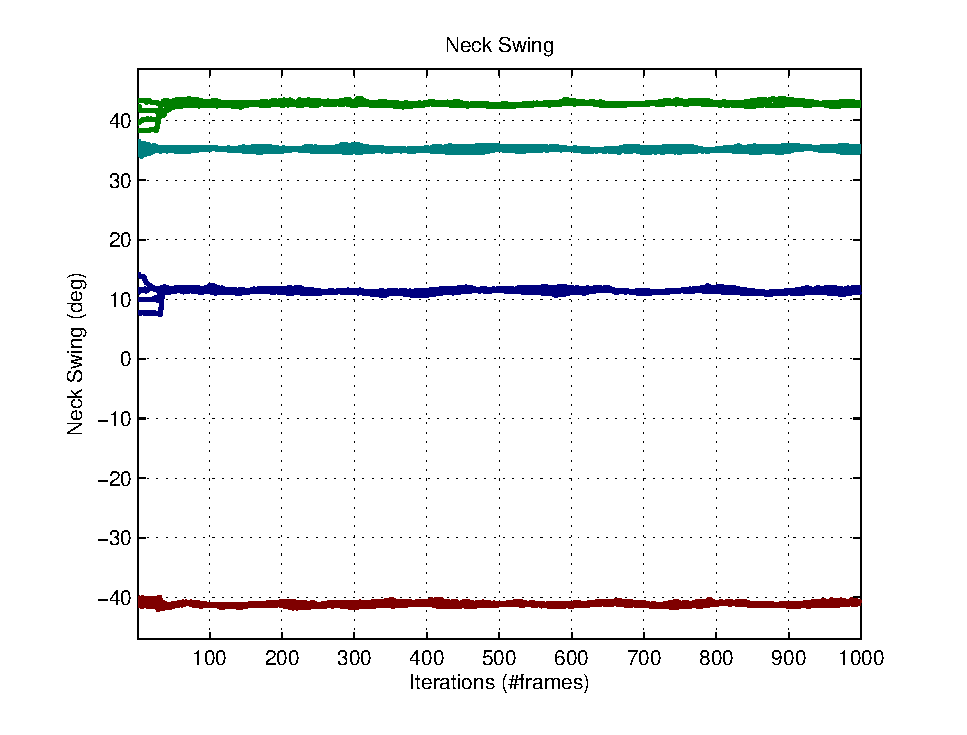
\includegraphics[width=0.32\linewidth]{images/results/neck_swing_offsets} &
 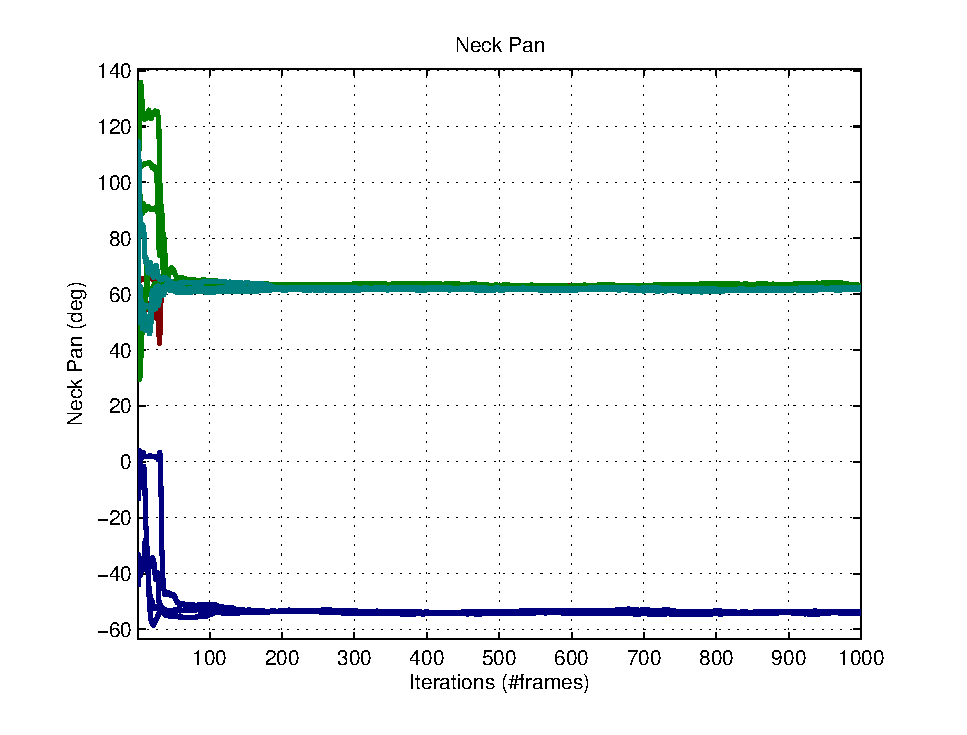
\includegraphics[width=0.32\linewidth]{images/results/neck_pan_offsets} \\
  a) $\delta_0$ - Neck Tilt & b) $\delta_1$ - Neck Swing & c) $\delta_2$ - Neck Pan \\
 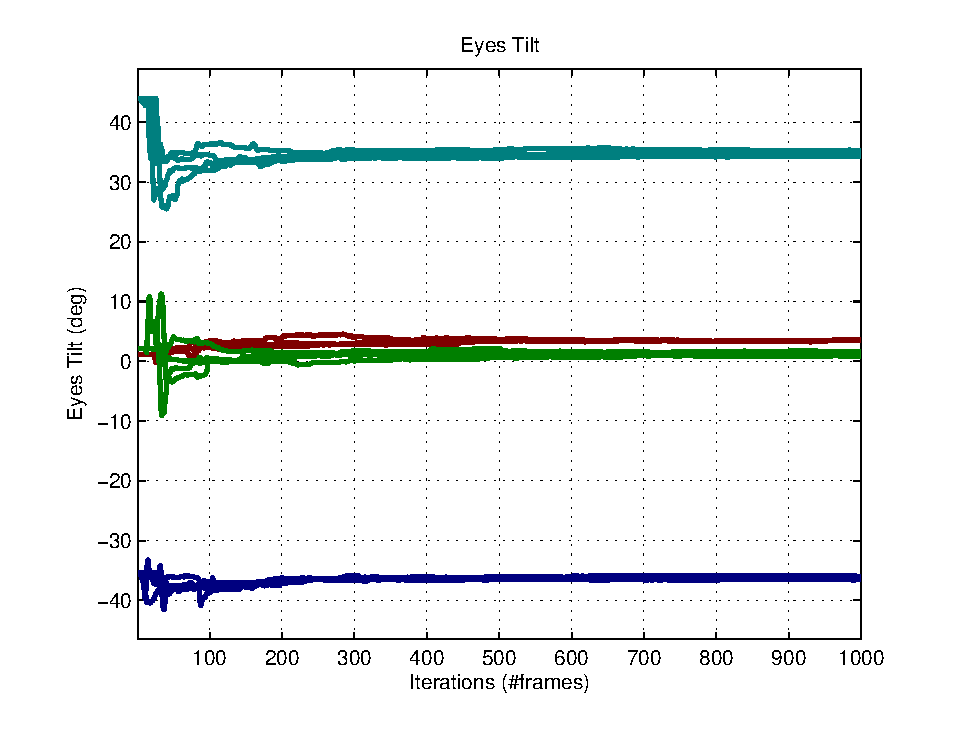
\includegraphics[width=0.32\linewidth]{images/results/eyes_tilt_offsets} &
 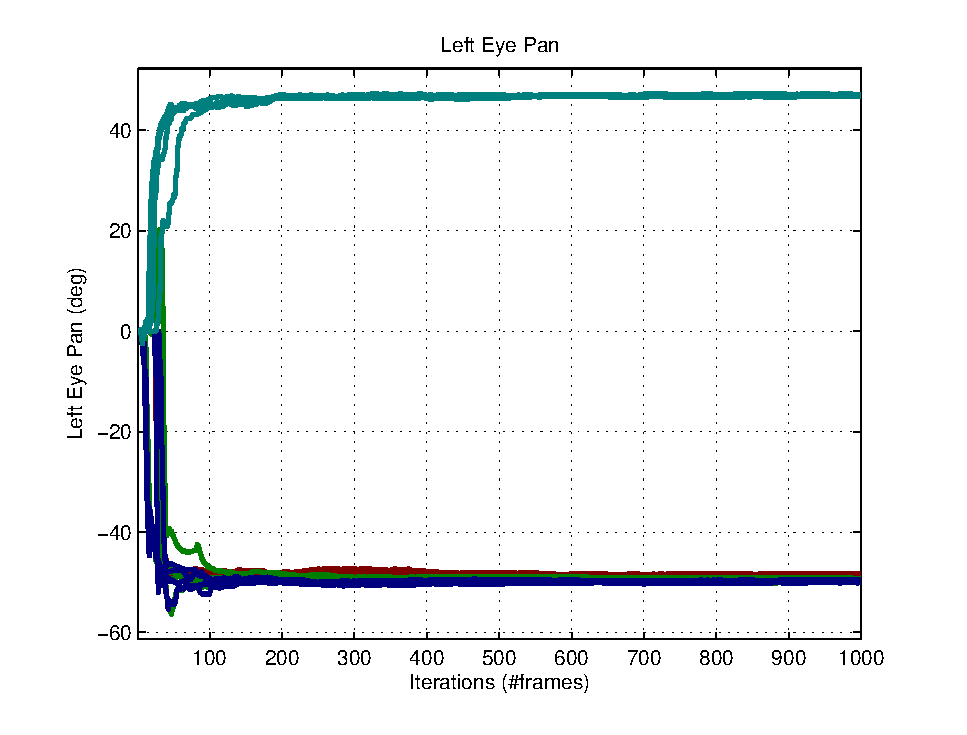
\includegraphics[width=0.32\linewidth]{images/results/left_eye_pan_offsets} & 
 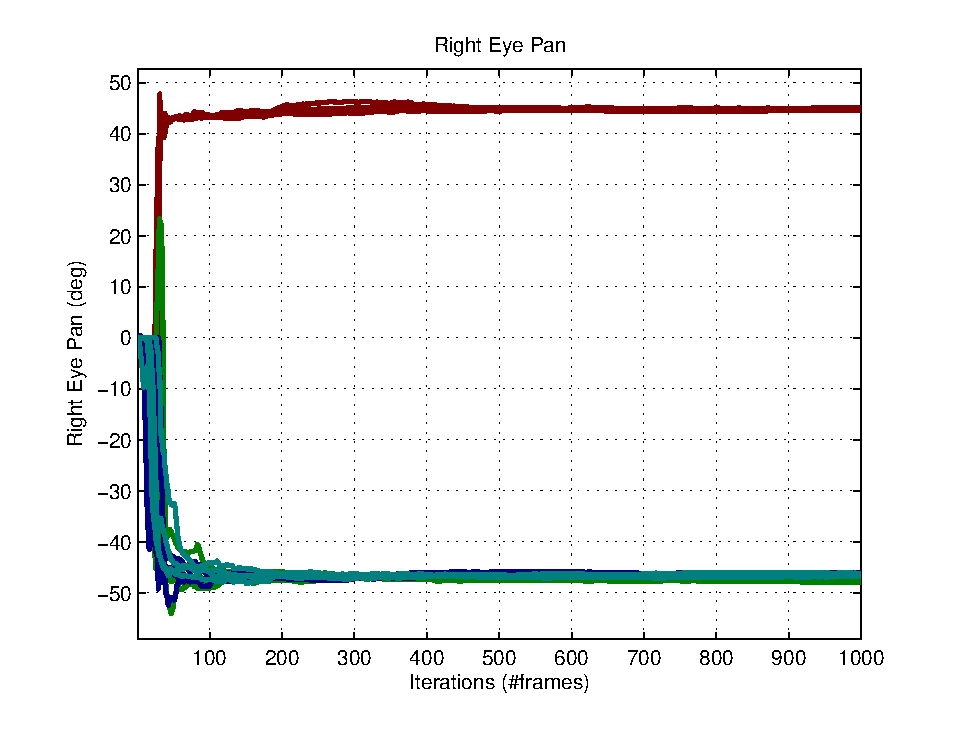
\includegraphics[width=0.32\linewidth]{images/results/right_eye_pan_offsets}\\
 d) $\delta_3$ - Eyes Tilt & e) $\delta_4$ - Left Eye Pan & f) $\delta_5$ - Right Eye Pan
\end{tabular}
\caption{Head calibration offsets estimates for $4$ experiments, with $5$ trials each, with the real robot: Experiment 1 (in red), Experiment 2 (in green), Experiment 3 (in blue) and Experiment 4 (in cyan)}
\label{fig:real_head_offsets_convergence}
\end{figure*}

\begin{table}
\centering
\begin{tabular}{lcccccc}
 \hline
 $\#$ Experiment & $\delta_0$(deg) & $\delta_1$(deg) & $\delta_2$(deg) & $\delta_3$(deg) & $\delta_4$(deg) & $\delta_5$(deg) \\
 \hline
$1$ (mean) & -41.16 & -40.92 & 62.35 & 3.49 & -48.61 & 44.79 \\
$1$ (std) & 0.44 & 0.25 & 0.30 & 0.06 & 0.24 & 0.23 \\
\hline
$2$ (mean) & -46.96 & 42.73 & 63.14 & 1.35 & -49.60 & -47.29 \\
$2$ (std) & 0.36 & 0.24 & 0.42 & 0.30 & 0.35 & 0.41 \\
\hline
$3$ (mean) & 42.81 & 11.43 & -53.95 & -36.18 & -49.82 & -46.27 \\
$3$ (std) & 0.38 & 0.32 & 0.19 & 0.23 & 0.24 & 0.26 \\
\hline
$4$ (mean) & 41.99 & 35.26 & 61.88 & 34.71 & 46.96 & -46.45 \\
$4$ (std) & 0.30 & 0.36 & 0.31 & 0.38 & 0.21 & 0.30 \\
 \hline
\end{tabular}
\caption{Mean and standard deviation values of the offsets estimates for all the experiments ($5$ trials for each experiment)}
\label{tab:real_head_offsets_convergence}
\end{table}

\subsubsection{Repeatability}

In figure \ref{fig:real_head_offsets_convergence}, we can see the system's repeatability considering that, for each experiment, it converged to very similar estimates under different operation of the robot. These results can be observed in table \ref{tab:real_head_offsets_convergence} where the maximum standard deviation value is $0.44$deg for all the four different configurations. As already mentioned in section \ref{sec:simulated_experiments} the system's repeatability is very important to guarantee the quality of the filter. 

During operation we noticed there were backlash zones in some of the joints, specially those carrying most of the weight. Within these backlash zones the encoders can not provide any measurements even though the joint is rotating in its motor shaft. However, the backlash was not reflected in the final estimates which shows that our system can adapt to sudden changes and perturbation that may occur during operation, mainly due to sensor fusion. The IMU and the cameras could perceive movement even though the encoders were telling the exact opposite. Sensor fusion is extremely useful to increase the robustness of the system in several situations where one or more sensors could fail. This case is a clear example of how multiple sensors integrated into a single architecture generate a better response than each one of them separated.

The accuracy of the head calibration system is hard to measure given the lack of ground-truth for each joint. Using the available sensors we measured the accuracy of the neck joints by comparing the real IMU's linear acceleration with the one predicted by the calibrated kinematic model of the robot head. In figure \ref{fig:real_head_imu} it is represented the real and predicted linear acceleration measurements for the three principal axis, for experiments $1$ and $2$, using only data from one trial for a better comprehension of the figure (these results are analogous for all the other experiments and trials).

\begin{figure*}
\centering
\begin{tabular}{ccc}
 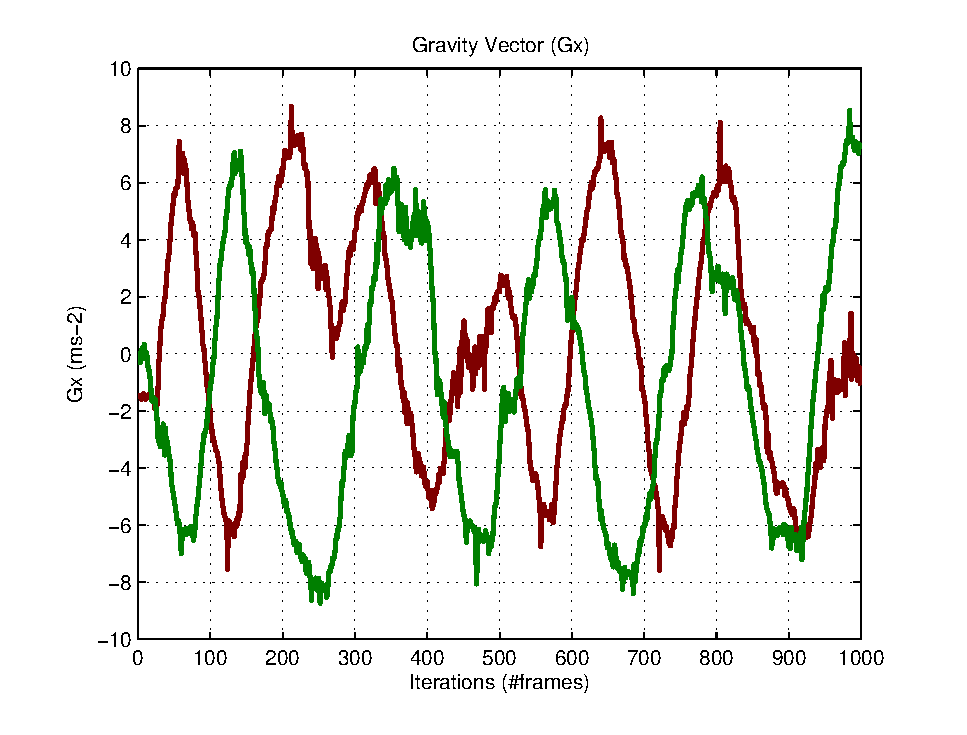
\includegraphics[width=0.32\linewidth]{images/results/gravity_vector_x} &
 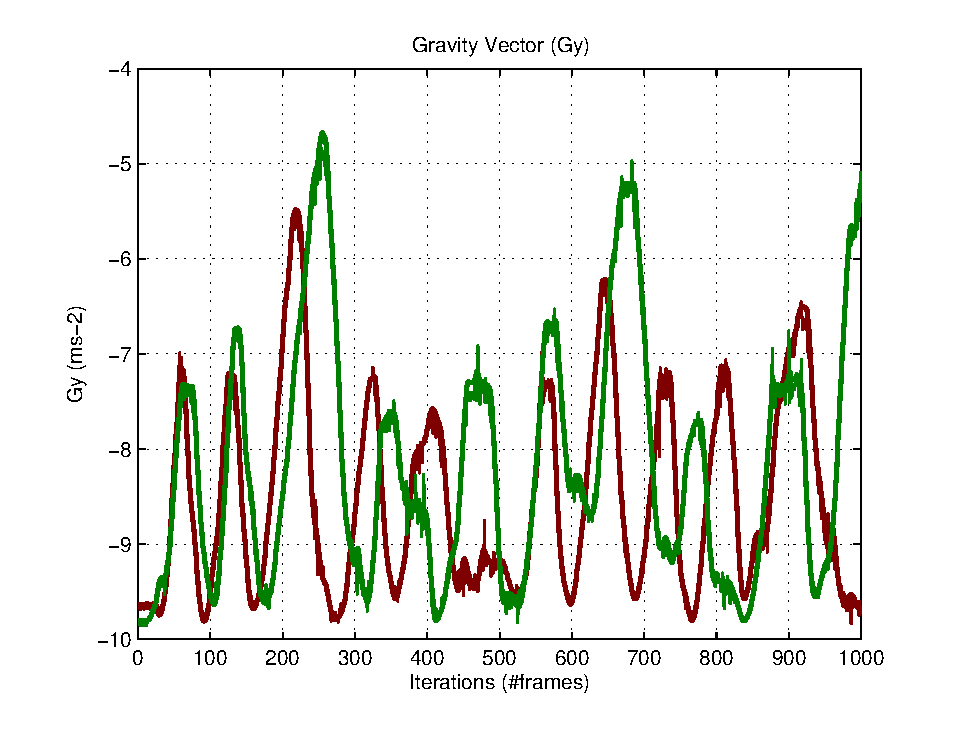
\includegraphics[width=0.32\linewidth]{images/results/gravity_vector_y} &
 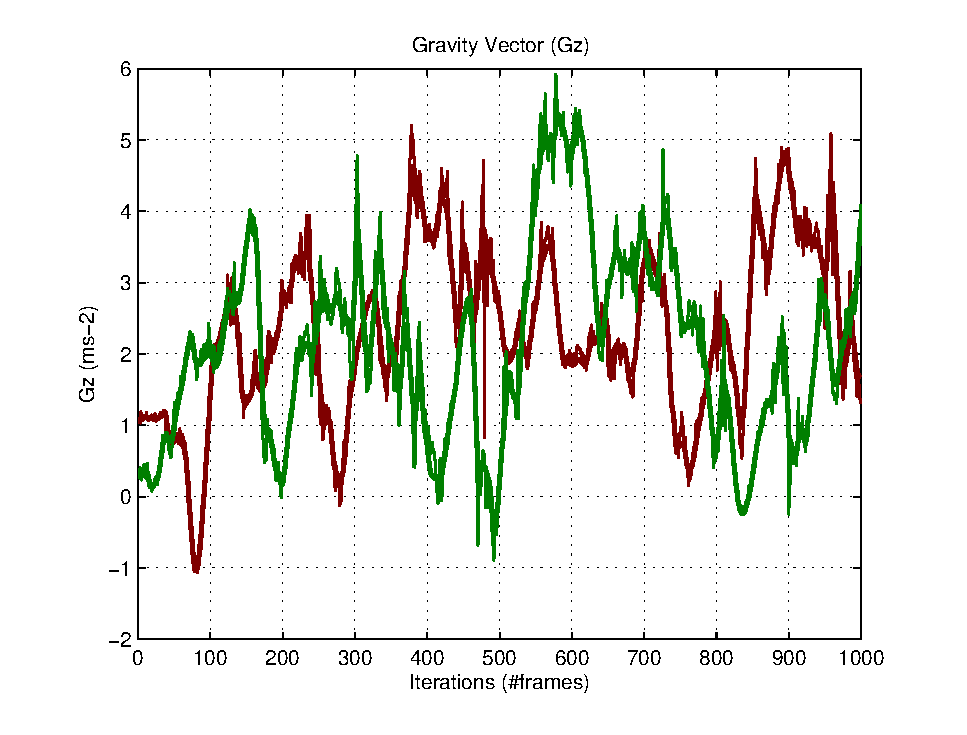
\includegraphics[width=0.32\linewidth]{images/results/gravity_vector_z} \\
 a) Gravity component $g_x$ &
 b) Gravity component $g_y$ &
 c) Gravity component $g_z$ \\
\end{tabular}
\caption{Real and predicted gravity vectors for Experiment $1$ (in red) and Experiment $2$ (in green), representing only one trial per experiment.}
\label{fig:real_head_imu}
\end{figure*}

As we can see the real and predicted signals are correctly aligned for different configurations of the head, with the prediction matching the real signal in more than $99\%$ ot the time. It is important to refer that it is assumed that the IMU is perfectly mounted on the top of the head, without any mounting error which may not be the case. In that case, the mounting error of the sensor will be reflected in the offsets estimates in order to approximate the real and predicted IMU signals. If the kinematic model can correctly predict the IMU measurements, then the offsets estimates converged to their correct values. 

\section{Experiments and Results}\label{sec:experiments_results}

In this section we will evaluate the proposed architecture for the head calibration system. We will perform simulated and real experiments to evaluate the system in terms of its accuracy and repeatability. The real experiments were performed using the iCub robotic platform, \cite{Metta08}, more specifically the head \cite{Beira06}. The iCub was developed in the context of the EU project RobotCub and was adopted by more than 20 laboratories worldwide. The full robot has 53 DOF with the head having 6 DOF from the neck to each of the eyes, as seen in figure \ref{fig:head_kinematic_model_prob_form}a).

For each joint the robot's head is equipped with relative encoders that are extremely precise but are unable to measure the absolute zero position of the joint. The head is also equipped with an Xsens IMU that measures the linear accelerations and angular velocities at a frequency of 100Hz. This sensor is placed on top of the head right before the eyes tilt joint, $\delta_3$, as seen in figure \ref{fig:head_kinematic_model_prob_form}a). Finally the head is equipped with two Pointgrey Dragonfly cameras, that work at 30Hz and provide RGB images with VGA resolution ($640\times480$pixel). These cameras have $4.7\times3.5$mm CCD sensors and a field of view of $87.3\degree$ (horizontal) and $70.8\degree$ (vertical). The cameras are the last sensors in the kinematic chain being affected by all the joints. The intrinsic parameters of the cameras were calibrated using the Bouguet Toolbox \cite{Bouguet08} and where the radial distortion was completely eliminated. The calibrated parameters are presented in table \ref{tab:intrinsic_parameters}.

\begin{table}
\centering
\begin{tabular}{ccc}
 \hline
 Parameter & Left Camera & Right Camera \\
 \hline
 Width (pixel) & $640$ & $640$\\
 Height (pixel) & $480$ & $480$ \\
 $f_x$ (pixel) & $332.706$ & $342.367$\\
 $f_y$ (pixel) & $382.658$ & $389.545$\\
 $c_x$ (pixel) & $348.316$ & $350.601$\\
 $c_y$ (pixel) & $241.872$ & $251.704$\\
 \hline\\
\end{tabular}
\caption{Intrinsic parameters of the cameras: resolution (Width and Height), focal lengths ($f_x$ and $f_y$) and optical centers ($c_x$ and $c_y$)}
\label{tab:intrinsic_parameters}
\end{table}

In order to validate the proposed architecture we performed simulated experiments where all the sensors measurements were simulated and fed to the system just like in the real case. For both cases, the simulated and real, we created multiple datasets. Each dataset contains information from all the sensors at every time step: the linear accelerations and angular velocities from the IMU, the motor encoders and stereo images from both cameras (or simulated image features in the simulation case).

The calibration procedure for the real case goes as follows: the motors are initialized at an arbitrary position and we start the data acquisition while randomly rotating the head, as seen in figure \ref{fig:head_calibration_procedure}. Several datasets were acquired either for the same encoders offsets and for different encoders offsets, to completely evaluate the system in terms of its accuracy and repeatability.

\begin{figure}
    \centering
    \begin{tabular}{ccc}
        \includegraphics[width=0.275\columnwidth]{images/pos_1} &  
        \includegraphics[width=0.275\columnwidth]{images/pos_2} & 
        \includegraphics[width=0.275\columnwidth]{images/pos_3} \\
        \includegraphics[width=0.275\columnwidth]{images/pos_4} &  
        \includegraphics[width=0.275\columnwidth]{images/pos_5} & 
        \includegraphics[width=0.275\columnwidth]{images/pos_6} \\
    \end{tabular}
    \caption{The head calibration procedure where the head is initialized at a random position and is rotated in order acquire data for the different experiments.}
    \label{fig:head_calibration_procedure}
\end{figure}

To initialize the system state uncertainty as well as the transition process noise we took into consideration the nature of the problem. We are estimating joint offsets that must be combined with the encoders values to provide calibrated measurements. We are initializing the system state with the first observations received from the encoders, as soon as the calibration system starts to run. For this reason, we have a large uncertainty at the beginning considering the physical limits of each joint. To ensure the system's convergence, the state's initial uncertainty must be large enough to include all the possible values the offsets could take. Therefore we initialized each offset uncertainty with a large value, $40$deg. The transition process noise was set to $0.05$deg, so it could adapt to sudden changes while keeping the estimates as constant as possible.

We analysed the noise levels that described each of the sensors' measurements, assumed to be zero mean Gaussian noise. The standard deviations values are represented in table \ref{tab:sensors_noise}.

\begin{table}
\centering
\begin{tabular}{ccc}
 \hline
 Sensor Measurement & Noise Std. Dev & Frequency (Hz) \\
 \hline
 Linear Acceleration & $0.0447m/s^2$ & $100$\\
  Angular Velocities & $0.5$deg/s & $100$\\
  Encoders & $0.028$deg & $>100$\\
  Image Features & $2$pixel & $30$\\
 \hline\\
\end{tabular}
\caption{Characterization of the Sensors}
\label{tab:sensors_noise}
\end{table}

In case of the image features, for this system we used the Harris Corner Detector \cite{Harris88} and Normalized Cross Correlation \cite{Briechle01} to track features between two consecutive images. Figure \ref{fig:harris_corners_tracking} shows an example of image features acquisition and corresponding tracking.

\begin{figure}
\centering
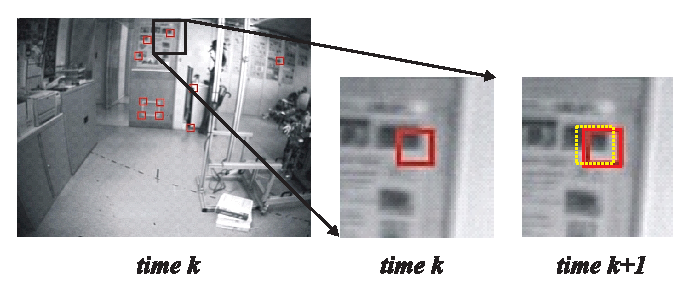
\includegraphics[width=0.75\columnwidth]{images/harris_corners_tracking}
\caption{Example of image features acquisition and tracking using the Harris Corner Detector and Normalized Cross Correlation between two images obtained at consecutive time instants $k$ and $k+1$.}
\label{fig:harris_corners_tracking}
\end{figure}

The features search in the next image was done within a limited region around the previous location of the features to reduce the computation time, assuming the images movement was small enough between two consecutive time instants.

\subsection{Simulated Experiments}\label{sec:simulated_experiments}

It is very difficult to measure the real absolute zero position of each motor joint considering there is no ground-truth for the real robot. One way to evaluate the calibration system in terms of its accuracy is by testing it with simulated experiments. Each experiment simulated the real conditions of the robot and introduced the same level of noise for each sensor according to the values in table \ref{tab:sensors_noise}. It is very important to create simulated environments whose conditions are similar to the real ones.

We performed $5$ experiments where we initialized each joint with different offset values. For each experiment we performed $5$ trials where we simulated the rotation of the robot head. Starting from an arbitrary position, the rotation step for an $i$th joint, $\delta_i^{step}$ was sampled from a Uniform Distribution $\delta_i^{step}\sim\mathcal{U}\left(-\theta,\theta\right)$ with $\theta=0.1$deg. These values were chosen in order to best replicate the real movement that was performed by hand. Between each two steps we sampled $50$ virtual image features by first generating their $3D$ coordinates, within a virtual scenario ranging from $250$mm to $4000$mm, for a certain time instant and calculating their matched coordinates in the consecutive instant by using the complete roto-translation of the head. The virtual image features used as measurements were then obtained by projecting each $3D$ generated point into the corresponding virtual images. Zero-mean Gaussian noise was added to the matched image coordinates, sampled from normal distribution with a standard deviation of $\sigma=2$pixel to simulate the real noise in the matching process.

The results obtained using the proposed algorithm are represented in table \ref{tab:head_offsets_convergence}, with the estimates for experiment $5$ illustrated in figure \ref{fig:head_offsets_convergence} as an example for analysis.

\begin{figure}
\includegraphics[width=0.975\columnwidth]{images/results/calibration_sim_exp_5}
\caption{Simulated experiments: head calibration offsets estimates for experiment $5$ ($5$ trials): Neck tilt $\delta_0$ (in orange), Neck swing $\delta_1$ (in yellow), Neck pan $\delta_2$ (in purple), Eyes tilt $\delta_3$ (in green), Left eye pan $\delta_4$ (in cyan) and Right eye pan $\delta_5$ (in red)}
\label{fig:head_offsets_convergence}
\end{figure}

\begin{table}
\centering
\begin{tabular}{lcccccc}
 \hline
 \# Experiment & $\delta_0$(deg) & $\delta_1$(deg) & $\delta_2$(deg) & $\delta_3$(deg) & $\delta_4$(deg) & $\delta_5$(deg) \\
 \hline
$1$ (ground-truth) & 13.00 & 24.00 & 38.00 & 30.00 & 18.00 & -9.00\\
$1$ (mean) & 13.02 & 23.97 & 38.01 & 31.40 & 17.99 & -7.27\\
$1$ (std) & 0.01 & 0.01 & 0.02 & 0.29 & 0.19 & 0.16 \\
$1$ (mean error) & 0.02 & 0.02 & 0.01 & 1.40 & 0.01 & 1.72\\
 \hline
$2$ (ground-truth) & -9.00 & -11.00 & -35.00 & -39.00 & -24.00 & -9.00\\
$2$ (mean) & -9.01 & -11.02 & -34.98 & -39.11 & -22.49 & -8.36\\
$2$ (std) & 0.01 & 0.02 & 0.03 & 0.41 & 0.17 & 0.40 \\
$2$ (mean error) & 0.01 & 0.02 & 0.01 & 0.12 & 1.50 & 0.63\\
 \hline
$3$ (ground-truth) & -41.00 & -3.00 & 30.00 & -8.00 & -35.00 & 0.00\\
$3$ (mean) & -40.95 & -3.01 & 30.00 & -8.26 & -32.80 & 0.40\\
$3$ (std) & 0.01 & 0.01 & 0.02 & 0.30 & 0.25 & 0.38 \\
$3$ (mean error) & 0.04 & 0.01 & 0.01 & 0.26 & 2.19 & 0.40\\
 \hline
$4$ (ground-truth) & -20.00 & -6.00 & 19.00 & 18.00 & 29.00 & 4.00\\
$4$ (mean) & -19.97 & -6.01 & 19.00 & 19.46 & 28.34 & 4.94\\
$4$ (std) & 0.01 & 0.01 & 0.02 & 0.21 & 0.18 & 0.20 \\
$4$ (mean error) & 0.02 & 0.01 & 1.01 & 1.46 & 0.65 & 0.94\\
 \hline
$5$ (ground-truth) & -14.00 & -5.00 & -56.00 & -43.00 & -33.00 & 12.00\\
$5$ (mean) & -13.99 & -5.01 & -56.01 & -43.14 & -31.55 & 11.67\\
$5$ (std) & 0.02 & 0.01 & 0.02 & 0.38 & 0.27 & 0.46\\
$5$ (mean error) & 0.00 & 0.01 & 0.00 & 0.14 & 1.44 & 0.32\\
 \hline\\
\end{tabular}
\caption{Simulated Experiments: ground-truth and statistical results of the head calibration offsets estimates for $5$ experiments, with $5$ trials each.}
\label{tab:head_offsets_convergence}
\end{table}

\subsubsection{Accuracy}

To evaluate the system in terms of its accuracy we compared the estimates with the ground-truth values represented in table \ref{tab:head_offsets_convergence}. As we can see the error between the real and estimated offsets is very low regardless of the starting position of the head. In this case we have a maximum error of $7\%$ (or $2.19$deg) for the left eye pan joint in experiment $3$. The eyes offsets are the ones presenting the largest errors which can be explained by the approximation taken for the calibration system, where we are assuming the world is static and all points are represented at infinity which may introduce parallax errors that are compensated by the system as errors in the joint space. However we can consider this approximation is still valid for small rotations in short steps between two consecutive time instants, considering our system presents an average error of $0.99$deg for the mentioned eyes joints ($\delta_4$ and $\delta_5$). All the other joints are able to converge to its correct values with much lower errors thus proving the accuracy of the proposed calibration system. 

By observing figure \ref{fig:head_offsets_convergence}, we can see that the system converges in less than $150$ iterations, which considering the lowest sensor runs at $30$Hz and the system works in real time, corresponds to a convergence in less than $5$s. This is very important since the robot can be rapidly calibrated before operation without consuming much of the operator's time. We can see each estimate remains almost constant after convergence, even if the head is continuously rotating. The low standard deviation values represented in table \ref{tab:head_offsets_convergence} show the stability of the system, keeping the estimates as constant as possible under different operation conditions, while the head was being rotated. This is extremely important considering the robot is being calibrated in an online fashion and should keep a well calibrated internal model at all times. 

\subsection{Real Experiments}\label{sec:real_experiments}

The validation of the proposed architecture was very important before testing it in the real robot. The quality of the previous results gave us confidence to test the calibration system in the real robot. Unfortunately, in the real case, there is no ground-truth for the real offsets of the robot. 

We started by performing four experiments (experiments $1$ to $4$) where we initialized the robot head at different arbitrary positions, with a full reset of the encoders between each experiment. For each experiment we performed five trials where we randomly rotated the robot head and eyes by hand during $33.33$ seconds ($1000$ iterations) so as to span most of the range of the robots joints. The mean and standard deviations for each experiment are represented in table \ref{tab:real_head_offsets_convergence}, with the estimates illustrated in figure \ref{fig:head_offsets_convergence_real} for experiment $4$ as an example for analysis.

\begin{figure}
\includegraphics[width=0.975\columnwidth]{images/results/calibration_exp_4}
\caption{Real experiments: head calibration offsets estimates for experiment $4$ ($5$ trials): Neck tilt $\delta_0$ (in orange), Neck swing $\delta_1$ (in yellow), Neck pan $\delta_2$ (in purple), Eyes tilt $\delta_3$ (in green), Left eye pan $\delta_4$ (in cyan) and Right eye pan $\delta_5$ (in red)}
\label{fig:head_offsets_convergence_real}
\end{figure}

\begin{table}
\centering
\begin{tabular}{ccccccc}
 \hline
 $\#$ Exp. & $\delta_0$(deg) & $\delta_1$(deg) & $\delta_2$(deg) & $\delta_3$(deg) & $\delta_4$(deg) & $\delta_5$(deg) \\
 \hline
$1$ (mean) & -41.44 & -41.13 & 62.52 & 3.49 & -48.41 & 44.63 \\
$1$ (std) & 0.60 & 0.68 & 0.73 & 0.11 & 0.35 & 0.27 \\
\hline
$2$ (mean) & -46.82 & 42.91 & 62.82 & 1.34 & -49.22 & -47.00 \\
$2$ (std) & 0.68 & 0.73 & 0.84 & 0.38 & 0.38 & 0.42 \\
\hline
$3$ (mean) & 42.87 & 11.41 & -53.97 & -36.17 & -49.68 & -46.13 \\
$3$ (std) & 0.70 & 0.68 & 0.77 & 0.25 & 0.19 & 0.21 \\
\hline
$4$ (mean) & 41.93 & 35.24 & 61.68 & 34.73 & 46.75 & -46.19 \\
$4$ (std) & 0.64 & 0.68 & 0.85 & 0.49 & 0.34 & 0.36 \\
 \hline\\
\end{tabular}
\caption{Real Experiments: mean and standard deviation values of the offsets estimates for all the experiments ($5$ trials for each experiment)}
\label{tab:real_head_offsets_convergence}
\end{table}

From the figure we can see that the system converged in less than $200$ iterations to very similar estimates under different operation conditions. These results show the capability of the system to correctly calibrate the offsets of the encoders regardless of their starting position, which is of utmost importance for any robotic platform. The low standard deviations for each experiments (maximum value of $0.85$deg), observed in table \ref{tab:real_head_offsets_convergence} also show the stability of the system, which keeps its estimates as constant as possible while the head was being rotated.  

The accuracy of the head calibration system is hard to measure in the real robot, given the lack of ground-truth for each joint. Using the available sensors we measured the accuracy of the neck joints by comparing the real IMU's linear acceleration with the one predicted by the calibrated kinematic model of the robot head. We performed four experiments (experiment $5$ to $8$), with one trial per each, where we initialized the head at different arbitrary positions with a full reset of the encoders between each experiment. After calibration was achieved, for each case the robotic head was homed to the calibrated zero position, using the calibrated offsets to define the absolute zero position of the head. The calibrated offsets and the corresponding recorded gravity vector readings are shown in tables \ref{tab:zero_position_offsets} and \ref{tab:zero_position}, respectively.

\begin{table}
\centering
\begin{tabular}{ccccccc}
 \hline
 $\#$ Exp. & $\delta_0$(deg) & $\delta_1$(deg) & $\delta_2$(deg) & $\delta_3$(deg) & $\delta_4$(deg) & $\delta_5$(deg) \\
 \hline
$5$ & -47.20 & 23.93 & -56.22 & -17.53 & -36.12 & 32.90 \\
$6$ & -34.14 & -35.17 & 49.23 & -19.21 & 38.83 & -40.09 \\
$7$ & 43.80 & -25.82 & 50.91 & -22.91 & 26.51 & -41.99 \\
$8$ & 43.39 & 28.47 & -44.03 & -21.15 & 23.43 & -39.52 \\
 \hline\\
\end{tabular}
\caption{Real Experiments: offsets estimates used to home the head to its zero position}
\label{tab:zero_position_offsets}
\end{table}

\begin{table}
\centering
\begin{tabular}{cccc}
 \hline
 $\#$ Experiment & $g_x$($m/s^2$) & $g_y$($m/s^2$) & $g_z$($m/s^2$) \\
 \hline
$5$ & -0.022 & -9.835 & -0.016 \\
$6$ & 0.034 & -9.844 & -0.096\\
$7$ & -0.102 & -9.829 & -0.091 \\
$8$ & -0.051 & -9.851 & -0.010 \\
 \hline\\
\end{tabular}
\caption{Real Experiments: gravity vector components in the zero position}
\label{tab:zero_position}
\end{table}

We can see that the gravity vector is practically vertical (with an accuracy of 99.99\%) for all four experiments. These results demonstrate the ability of the system to converge to a solution which agrees with the absolute gravity readings, when started in completely different head configurations, thus correctly setting the absolute zero position of the head. After homing to the zero position, for each experiment, we applied a rectangular signal to the neck tilt joint (joint $\delta_0$) in order to compare the real and predicted observations for the gravity vector. The comparison is represented in figure \ref{fig:real_predicted_imu} for experiment $5$ as an example for analysis.

\begin{figure}
 \includegraphics[width=0.975\columnwidth]{images/results/gravity_all}
\caption{Real (red dashed) and predicted (blue solid) gravity vectors for Experiment $5$, with homing to zero position after convergence and response to rectangular signal applied to the first joint, neck tilt.}
\label{fig:real_predicted_imu}
\end{figure}

Figure \ref{fig:real_predicted_imu} correctly shows a leaning forward and backwards pattern, after iteration $1700$, corresponding to the signal applied to the first joint. After convergence of the filter, the predicted and real observations for the gravity vector are correctly aligned, with the prediction matching the real signal in more than $99.9\%$ ot the time. It is important to refer that the IMU is assumed to be perfectly mounted on the top of the head, without any mounting error which may not be true. In that case, the mounting error of the sensor will be reflected in the offsets estimates in order to approximate the real and predicted IMU signals.

\subsubsection{Repeatability}

To better analyse the repeatability of the system, we performed experiment $9$ where we ran the algorithm with the robot head started in six different configurations without a full reset of the encoders, meaning the offsets were the same
for all trials. Figure \ref{fig:offsets_repeatability} shows the convergence of the offset estimates in each trial, with the mean value taken in the last $500$ iterations shown in table \ref{tab:offsets_repeatability} along with the standard deviation of the estimates for all trials. The results show the estimates converging to similar values for different trials, thus empirically proving the robustness of the proposed method to very different starting conditions. The system's repeatability is extremely important to guarantee the quality of the filter, allowing the correct operation of the platform.

\begin{figure}
 \includegraphics[width=0.975\columnwidth]{images/results/repeatability_all}
\caption{Repeatability: head calibration offsets estimates for experiment $9$, with $6$ trials, without a full reset of the encoders, showing the repeatability of the system}
\label{fig:offsets_repeatability}
\end{figure}

\begin{table}
\centering
\begin{tabular}{ccccccc}
 \hline
 $\#$ Trial & $\delta_0$(deg) & $\delta_1$(deg) & $\delta_2$(deg) & $\delta_3$(deg) & $\delta_4$(deg) & $\delta_5$(deg) \\
 \hline
$1$ & -43.8 & 31.7 & -50.2 & -2.1 & 37.3 & -42.4 \\
$2$ & -43.4 & 32.6 & -52.7 & -3.4 & 35.5 & -43.7 \\
$3$ & -43.4 & 31.4 & -50.9 & -1.5 & 36.9 & -40.4 \\
$4$ & -43.1 & 32.0 & -52.0 & -3.9 & 37.4 & -42.2 \\
$5$ & -43.4 & 32.8 & -51.1 & -2.3 & 39.8 & -42.1 \\
$6$ & -43.0 & 33.0 & -52.9 & -3.9 & 35.7 & -41.6 \\
 \hline
mean & -43.57 &  32.31 & -50.54 & -2.72 & 36.85 & -42.20 \\
std & 0.28 & 0.64 & 1.07 & 1.02 & 1.54 & 1.08 \\
 \hline \\
\end{tabular}
\caption{Repatability: mean values of the offsets estimates for experiment $9$, with $6$ trials, without a full reset of the encoders}
\label{tab:offsets_repeatability}
\end{table}

It is worth noting, in figure \ref{fig:offsets_repeatability}, that immediately after the first iteration the system has already assimilated the first reading of the accelerometer. Since different head configurations can provide the same accelerometer readings (e.g. different pan angles with a fully upright head), the initial measurements are not enough to converge to the final configuration nor do they provide any information about the eye joints. The head movements are required to disambiguate these multiple solutions and provide the final offsets values, as seen by the rapid convergence of the filter after rotating the head.

During operation we noticed there were backlash zones in some of the joints, specially those carrying most of the weight. Within these backlash zones the encoders can not provide any measurements even though the joint is rotating in its motor shaft. However, the backlash was not reflected in the final estimates which shows that our system can adapt to sudden changes and perturbation that may occur during operation, mainly due to sensor fusion. The IMU and the cameras could perceive movement even though the encoders were telling the exact opposite. Sensor fusion is extremely useful to increase the robustness of the system in several situations where one or more sensors could fail. This case is a clear example of how multiple sensors integrated into a single architecture generate a better response than each one of them separated.
\section{Conclusions}\label{sec:conclusions}

%This work focus on the complete calibration of the kinematic model of a robot's head using only information from embedded sensors and non-linear filtering techniques. We have designed and implemented a calibration system at a kinematic level to be applied when the joints are equipped with relative encoders. The proposed system is able to rapidly estimate the offsets for each joint by using a non-linear filter together with information from the encoders, the IMU and the cameras. The sensor fusion allows the correct estimation of the joint offsets under any circumstance turning the system more robust and extremely adaptable. The results show an accurate calibration system that can easily calibrate a kinematic platform within a few iterations, which is important when the robotic platform is used on a daily basis, requiring a calibration procedure before executing a task.

%The proposed system was designed to be as general as possible so it could easily calibrate almost any kinematic model using information from the embedded sensors only. Although, for certain configurations of the joints, it is impossible to correctly calibrate the offsets due to observability problems. The system can not estimate the offsets of two or more consecutive joints that rotate over the same axis, affecting all the sensors' measurements at once. Such a structure allows for multiple combinations of the joints, leading to the exact same orientation of the end-effector, which results in a wide range of value to which the offsets can converge. This observability problem is a major limitation of our system that can not be solved at a software level and must be always considered. Nevertheless, our system is able to calibrate any other kinematic model regardless of its joints' orientation and chain order, which makes this an extremely useful tool for robotics.

We have presented a robust, online calibration system for
the joints of a robot head. This calibration system is able to provide accurate estimates for the offsets of the joints, irrespective of the head initial configuration.
The approach uses information from the embedded inertial
sensor, the relative encoders of the joints and vision and it performs robustly in the presence of noise and disturbances such as backlash in some joints. As opposed to other methods, our approach is very efficient and calibration can be achieved in a matter of a couple of seconds and a few movements of the robot head.

Our work provides a way of correctly initializing the
robot, no matter what the robot’s starting position might
be, which is absolutely mandatory before the robot can
engage in complex tasks. We present results with the iCub
head, as humanoid robots represent the best metaphor of
complex sensorimotor chains. Nevertheless, the proposed system was designed to be as general as possible so it could easily calibrate almost any kinematic model, if fully observable, using information from the embedded sensors only.

The relevance of this calibration procedure is that it allows the system to maintain an accurate internal model of its sensorimotor chains. These models are key for the control of humanoid robots, as the complexity of the tasks and diversity of the operational environments may be overwhelming. Instead, these models allow the system to contrast its observations to model-based predictions, substantially simplifying certain tasks, a mechanism similar to the one presumably used by humans.
%\input{appendices}

% use section* for acknowledgement
%\section*{Acknowledgment}

%The authors would like to thank...

\printbibliography

%\begin{thebibliography}{1}
%\bibitem{IEEEhowto:kopka}
%H.~Kopka and P.~W. Daly, \emph{A Guide to \LaTeX}, 3rd~ed.\hskip 1em plus
%  0.5em minus 0.4em\relax Harlow, England: Addison-Wesley, 1999.

%\end{thebibliography}

%\begin{IEEEbiography}[{\includegraphics[width=1in,height=1.25in,clip,keepaspectratio]{images/nuno}}]{Nuno Moutinho}
Nuno Moutinho is a PhD student and researcher at the Dept. of Electrical and Computer Engineering of the Faculty of Engineering at IST, the Faculty of Engineering in the Technical University of Lisbon.

His main research interests focus on computer vision applied to robotic systems, self-calibration mechanisms for robotic platforms, visual SLAM, augmented reality and Expected Perception mechanisms. He has published works on Expected Perception, kinematic self-calibration of robotic platforms and automatic calibration of stereo systems in several international conferences. He has been participating in many national and international projects involving both academic and industrial partners. He is also the co-founder and CTO of boomApp, a computer vision startup specialized in large scale video recognition algorithms.
\end{IEEEbiography}

\begin{IEEEbiography}[{\includegraphics[width=1in,height=1.25in,clip,keepaspectratio]{images/ricardo}}]{Ricardo Ferreira}
\end{IEEEbiography}

\begin{IEEEbiography}[{\includegraphics[width=1in,height=1.25in,clip,keepaspectratio]{images/gaspar}}]{Jose Gaspar}
\end{IEEEbiography}

\begin{IEEEbiography}[{\includegraphics[width=1in,height=1.25in,clip,keepaspectratio]{images/alex}}]{Alexandre Bernardino}

Alexandre Bernardino is an Associate Professor at the Dept. of Electrical and Computer Engineering of the Faculty of Engineering at IST, the Faculty of Engineering in the Technical University of Lisbon.
He teaches on the scientific area of decision systems and control, in courses involving signal and image processing, automation and robotics, modeling and control, artificial intelligence and machine learning.

He's a senior researcher at ISR-Lisboa (the Institute for Systems and Robotics of IST), member of LARSyS (Laboratory of Robotics, Systems of Engineering and Science), and co-director of VisLab, the Computer and Robot Vision Laboratory.
His main research interests focus on the application of computer vision, cognitive science, control theory and machine learning to advanced robotic and surveillance systems.
He has published works on foveal sensors, visual attention and stereo, image feature extraction, binocular head control, image based tracking and identification, learning object affordances, sensorimotor coordination, human activity recognition, among other topics. He has been participating in many national and international projects involving both academic and industrial partners.
\end{IEEEbiography}

% that's all folks
\end{document}


